\section{Results}\label{sec:results}

\subsection{Descriptive patterns}

Table~\ref{tab:descriptives} summarises the estimation sample. Mean GER is 30.4\%, with a standard deviation of 8.8 points. The distribution is wide and slightly left-skewed: the median (30.6\%) is close to the mean, but the minimum (16.9\%) is further below the median than the maximum (47.0\%) is above it. Fourteen States are below 30\%, and none has reached 50\%. College density averages 31.0 colleges per lakh, with a range from 7 in Bihar to 66 in Karnataka. PTR averages 24.6 and ranges from 14 in Tamil Nadu to 64 in Bihar. GPI averages 1.06, with ten States below parity and seven at or above 1.2.

\begin{table}[htbp]
\centering
\small
\caption{Descriptive statistics, 28 States, 2021-22. Average enrolment per college is shown for reference and is used only in a robustness model. Source: \texttt{table01\_summary\_statistics.csv}.}
\label{tab:descriptives}
\begin{tabular}{@{}lrrrrr@{}}
\toprule
Variable & Mean & SD & Min & Median & Max \\
\midrule
GER (\%) & 30.4 & 8.8 & 16.9 & 30.6 & 47.0 \\
College density (per lakh 18--23) & 31.0 & 13.7 & 7.0 & 29.0 & 66.0 \\
Pupil--teacher ratio & 24.6 & 11.5 & 14.0 & 22.5 & 64.0 \\
Gender Parity Index & 1.06 & 0.15 & 0.88 & 1.02 & 1.44 \\
Average enrolment per college & 800 & 394 & 413 & 668 & 2,088 \\
\bottomrule
\end{tabular}
\end{table}

Table~\ref{tab:correlations} reports Pearson and Spearman correlations. Density has the strongest positive association with GER (\(r = 0.712\); \(\rho = 0.751\)), followed by PTR with a negative association (\(r = -0.612\); \(\rho = -0.645\)). GPI is weakly associated (\(r = 0.189\); \(\rho = 0.173\)), and average enrolment per college is negatively associated (\(r = -0.460\)). Density and PTR are themselves correlated at \(-0.66\), which is why the multivariate density coefficient is smaller than the bivariate slope.

\begin{table}[htbp]
\centering
\small
\caption{Correlations with GER, 28 States, 2021-22. Pearson and Spearman coefficients; the Spearman coefficient for average enrolment is not reported because the variable is used only as a robustness check. Source: \texttt{table02\_correlations.csv} and \texttt{table02b\_spearman.csv}.}
\label{tab:correlations}
\begin{tabular}{@{}lrr@{}}
\toprule
Variable & Pearson \(r\) & Spearman \(\rho\) \\
\midrule
College density & 0.712 & 0.751 \\
Pupil--teacher ratio & $-0.612$ & $-0.645$ \\
Gender Parity Index & 0.189 & 0.173 \\
Average enrolment per college & $-0.460$ & --- \\
\bottomrule
\end{tabular}
\end{table}

\begin{figure}[htbp]
\centering
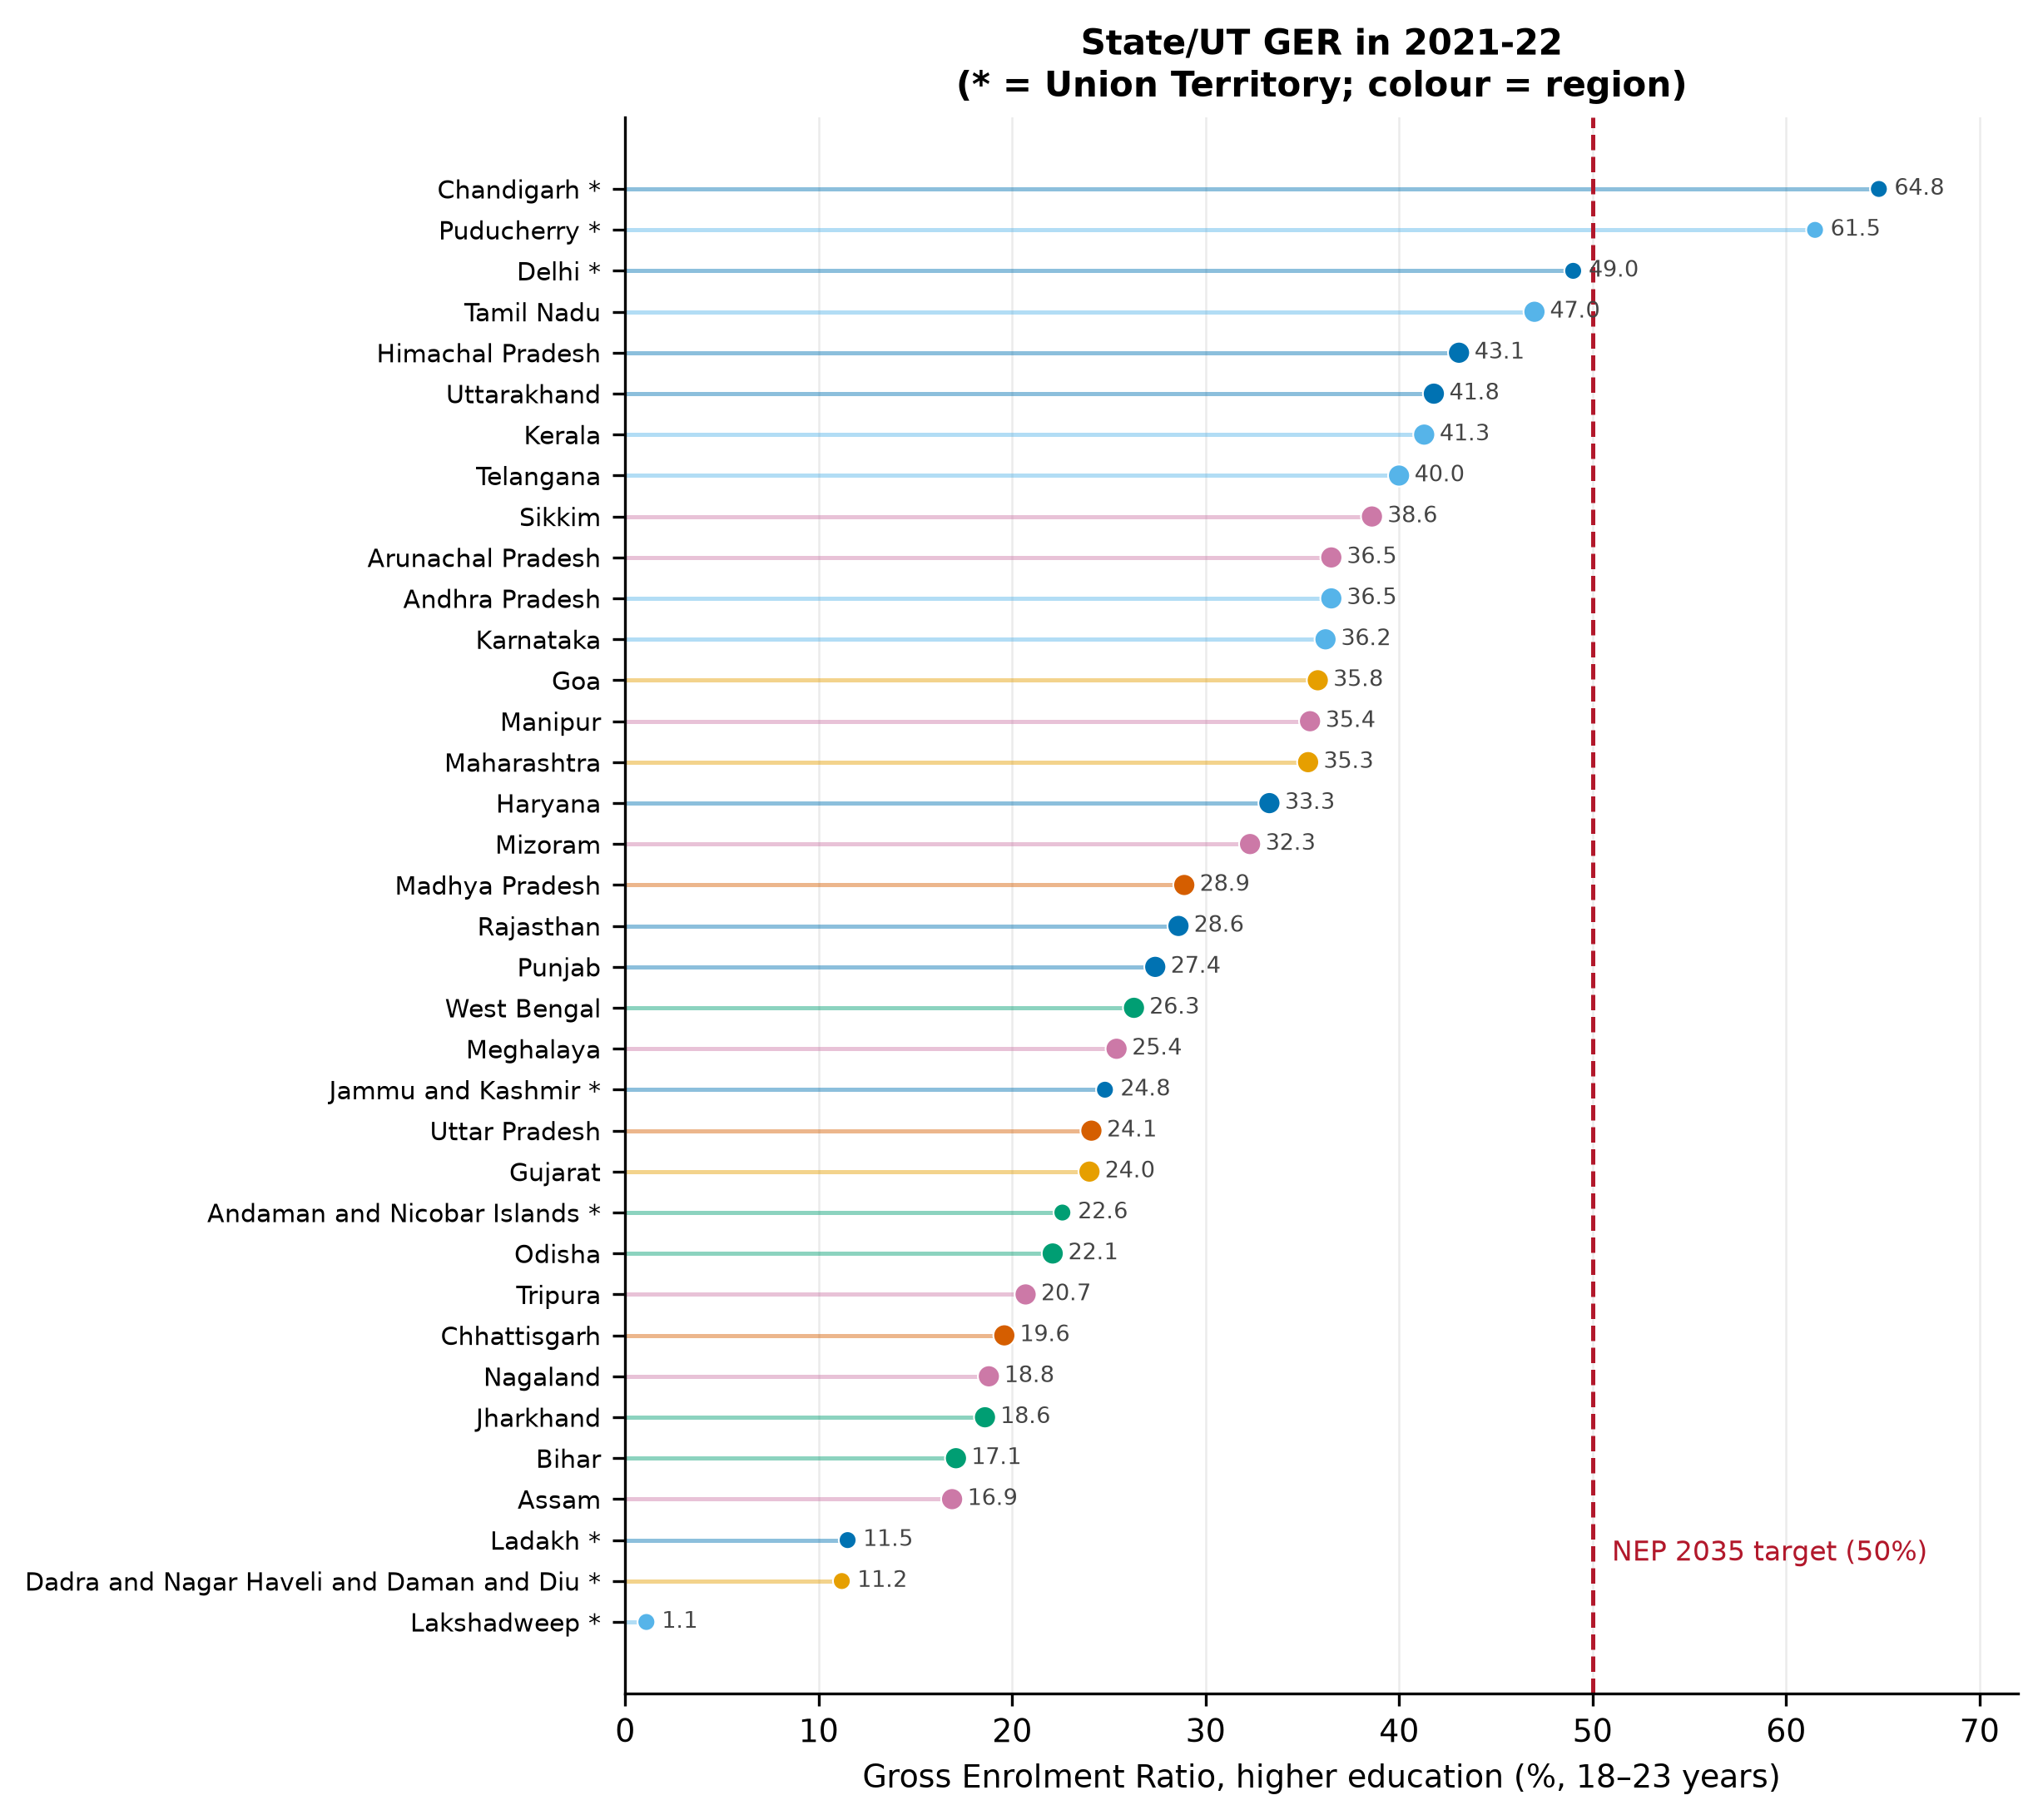
\includegraphics[width=0.86\linewidth]{fig01_ger_ranked.png}
\caption{State and Union Territory GER in 2021-22, ranked. The southern and hilly States cluster at the top; the Gangetic plain and the Northeast contain most of the low-GER units. Union Territories are shown for context but are excluded from estimation. Source: \texttt{fig01\_ger\_ranked.png}.}
\label{fig:ranked}
\end{figure}

Figure~\ref{fig:ranked} shows the full ranking of 36 units. Tamil Nadu (47.0), Himachal Pradesh (43.1), Uttarakhand (41.8), Kerala (41.3) and Telangana (40.0) lead the States. Assam (16.9), Bihar (17.1), Jharkhand (18.6), Nagaland (18.8), Chhattisgarh (19.6), Tripura (20.7), Odisha (22.1) and Uttar Pradesh (24.1) trail. The UTs are a separate distribution: Chandigarh (64.8), Puducherry (61.5) and Delhi (49.0) are high, while Dadra and Nagar Haveli and Daman and Diu (11.2) is the lowest unit in the file.

\begin{figure}[htbp]
\centering
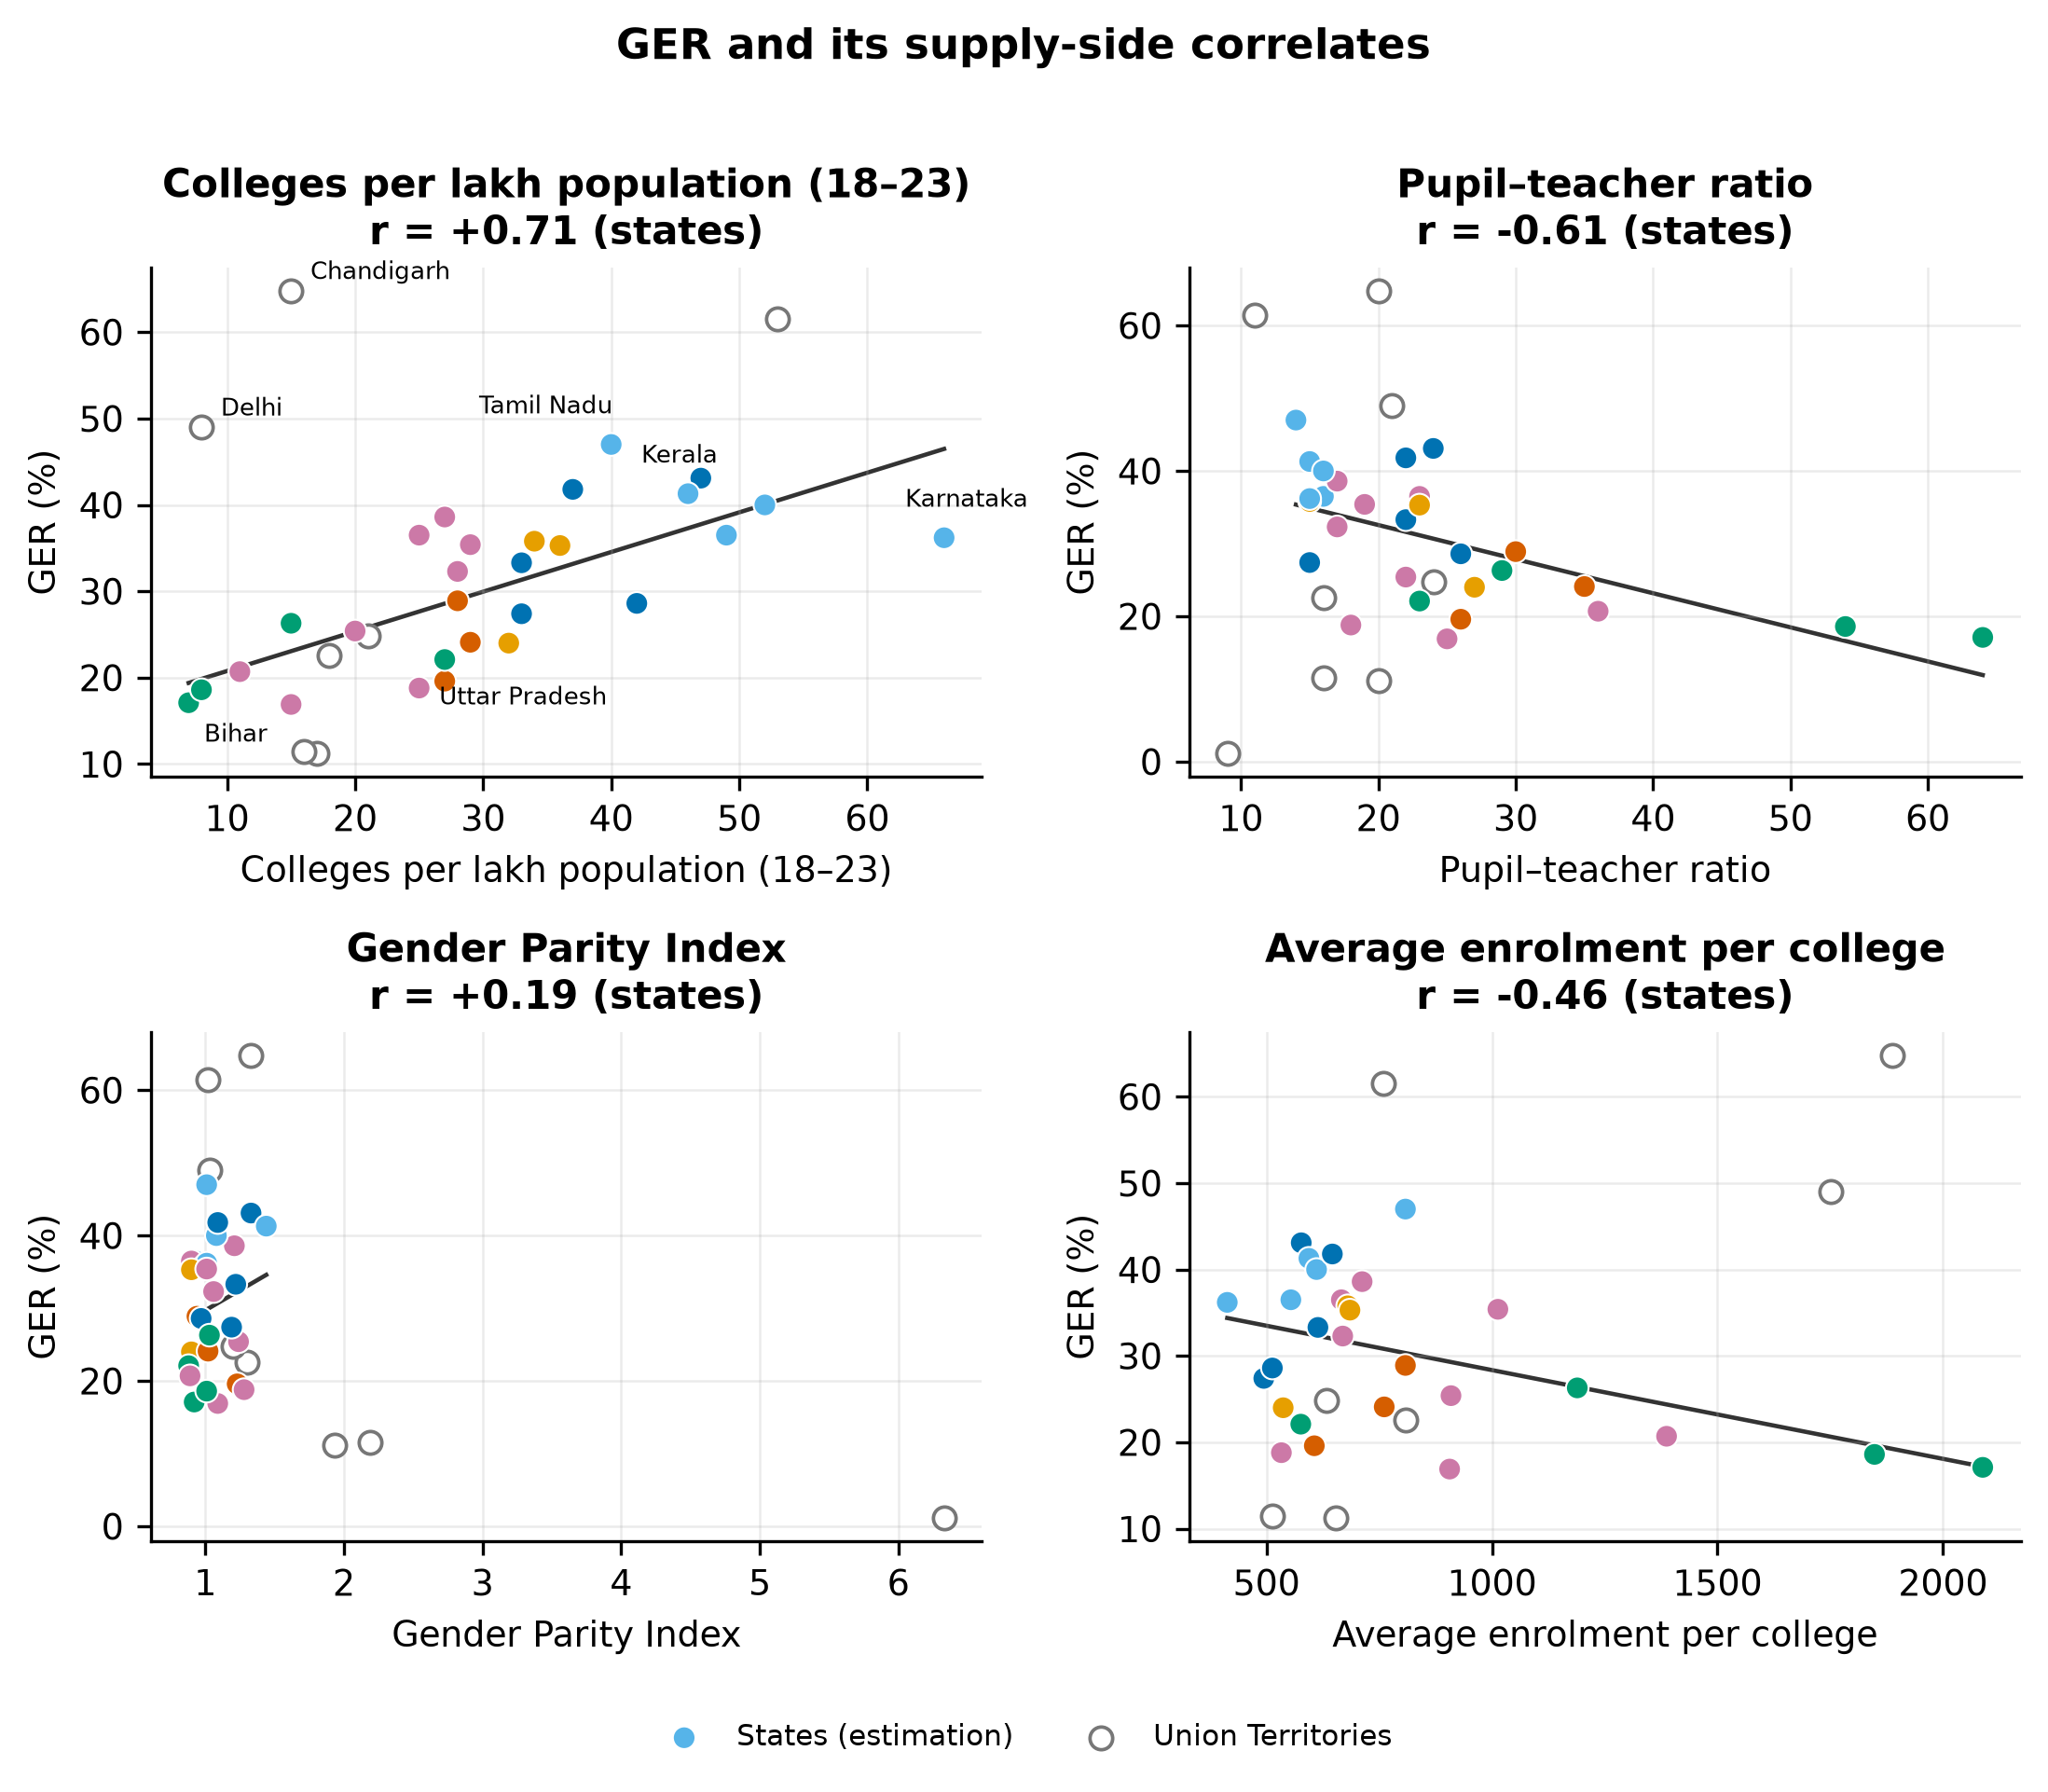
\includegraphics[width=\linewidth]{fig02_correlates.png}
\caption{GER against the four candidate correlates, 28 States, 2021-22. Density is positively associated, PTR negatively, GPI weakly, and average enrolment per college negatively. Source: \texttt{fig02\_correlates.png}.}
\label{fig:correlates}
\end{figure}

Figure~\ref{fig:correlates} makes the bivariate patterns visible and also shows why a multivariate model is needed. The density relationship is tight but has notable exceptions: Karnataka has the highest density (66) but a GER of only 36.2, while Tamil Nadu reaches 47.0 with a density of 40. The PTR relationship is negative but is driven partly by the low-density, high-PTR States. The GPI panel is almost flat. Average enrolment per college is negatively related to GER, which is a warning that college size is not a quality proxy: Bihar combines the largest average college (2,088 students) with the lowest density and a GER of 17.1.

\begin{figure}[htbp]
\centering
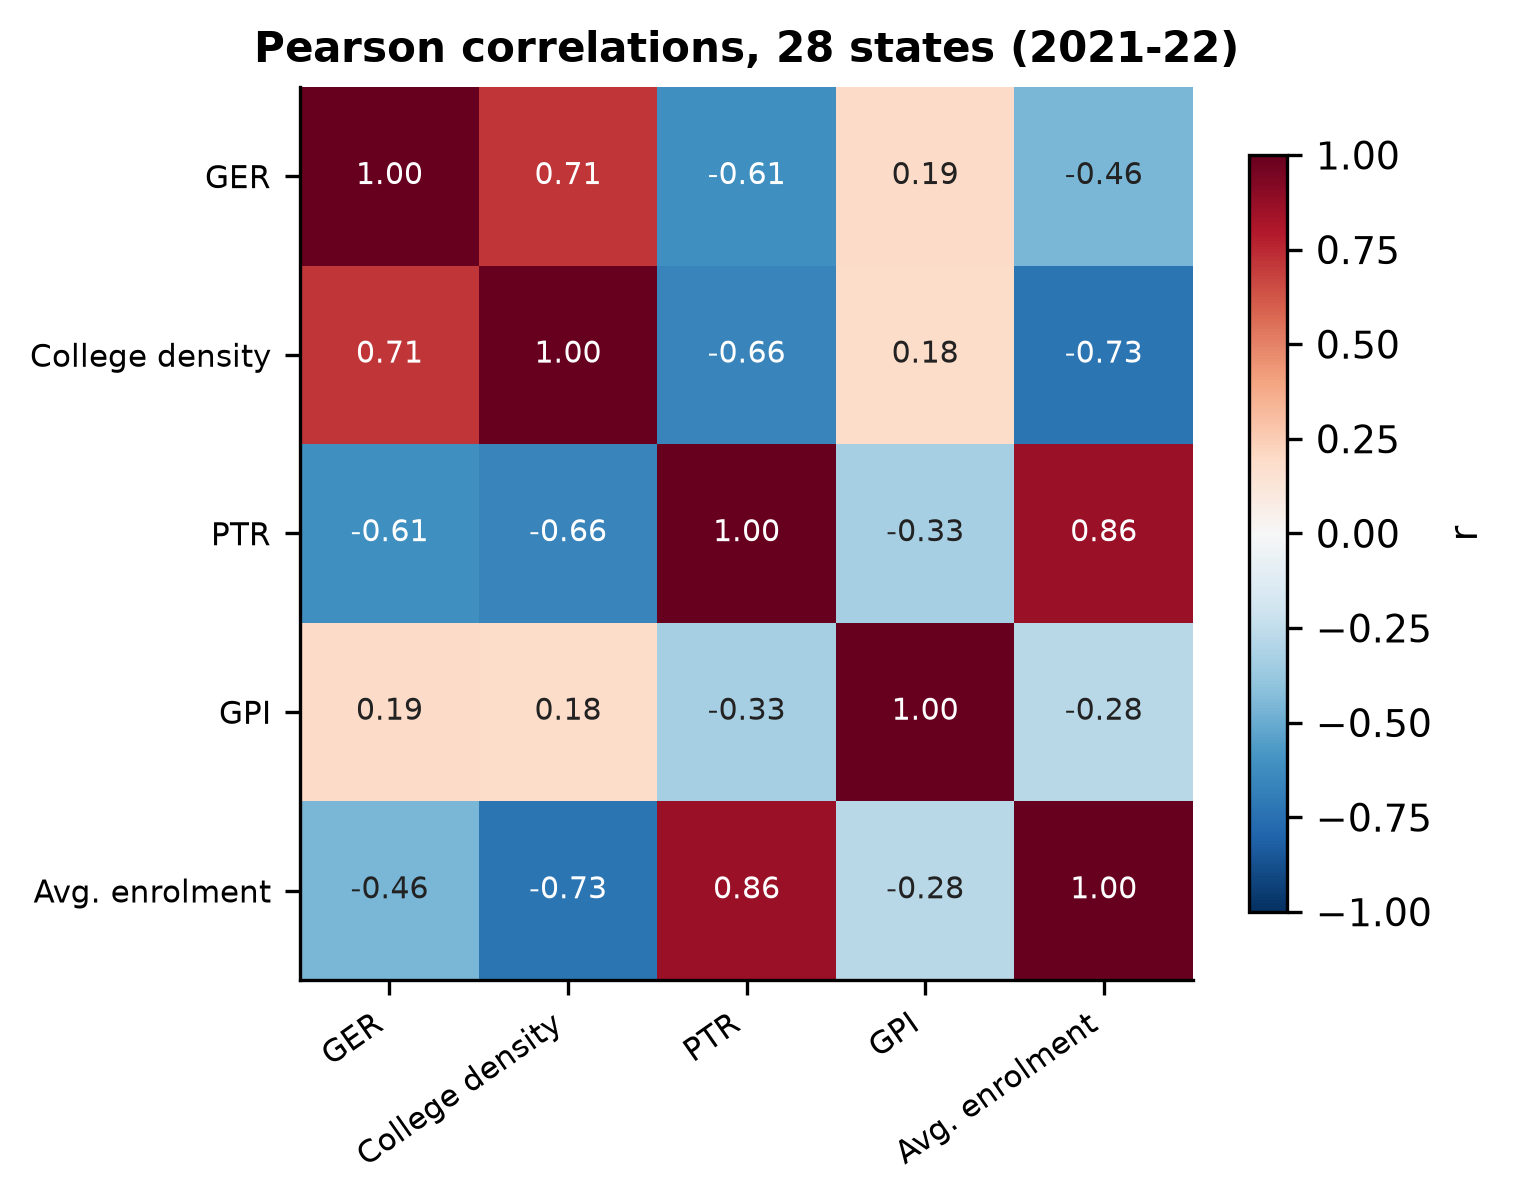
\includegraphics[width=0.82\linewidth]{fig03_correlation_heatmap.png}
\caption{Pearson correlation matrix for GER and its correlates, 28 States, 2021-22. Density and PTR are strongly negatively correlated; GPI is weakly correlated with both. Source: \texttt{fig03\_correlation\_heatmap.png}.}
\label{fig:heatmap}
\end{figure}

\begin{figure}[htbp]
\centering
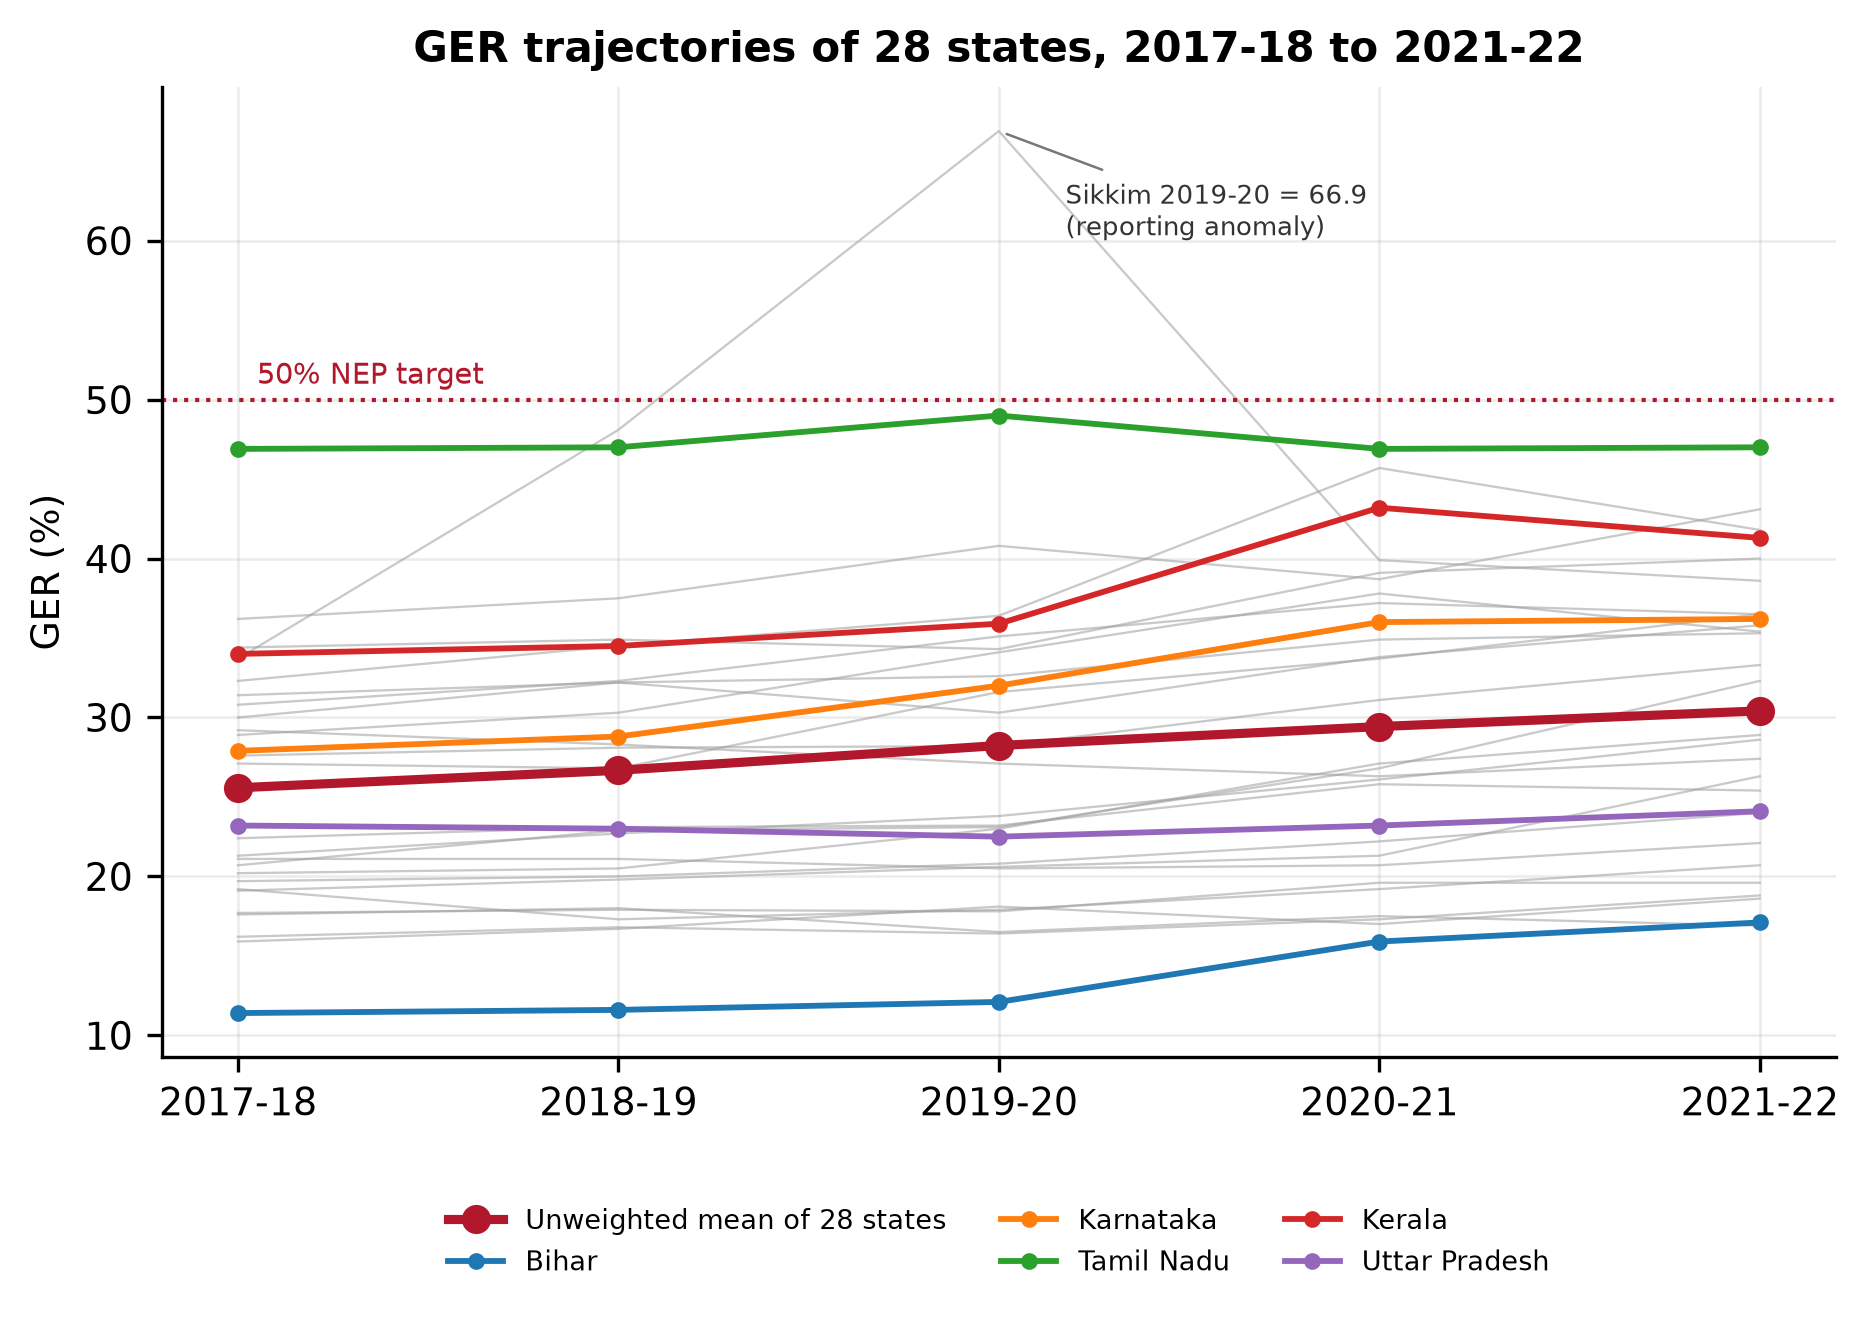
\includegraphics[width=\linewidth]{fig04_trajectories.png}
\caption{GER trajectories, 2017-18 to 2021-22. Most States improved, but the gap between the top and bottom groups persisted. The 2019-20 Sikkim observation is annotated as a reporting anomaly. Source: \texttt{fig04\_trajectories.png}.}
\label{fig:trajectories}
\end{figure}

Figure~\ref{fig:heatmap} confirms the density--PTR collinearity and the weak GPI--GER association. Figure~\ref{fig:trajectories} shows that the level differences are persistent: the States at the top in 2017-18 are mostly at the top in 2021-22, and the bottom group improves from a lower base. This persistence is why a cross-sectional model has explanatory power and why a change-based projection is more defensible than a level forecast.

\subsection{Model comparison}

Table~\ref{tab:tuning} reports the hyper-parameter grids and the selected values. Table~\ref{tab:models} reports the model comparison. The polynomial ridge model has the lowest LOOCV RMSE (5.96) and the highest LOOCV \(R^2\) (0.525). OLS with college size is second (6.27; 0.474), followed by ridge with college size (6.42; 0.449), ridge with three indicators (6.74; 0.392) and OLS with three indicators (6.86; 0.370). The tuned tree (7.39; 0.269) and tuned \(k\)-NN (7.59; 0.229) are worse than OLS, despite much higher in-sample \(R^2\) (0.702 and 0.660). The baseline is worst (8.97; $-0.075$).

\begin{table}[htbp]
\centering
\caption{Hyper-parameter grids, selection rule and selected values. The ridge penalty \(\lambda\) corresponds to \texttt{alpha} in \texttt{RidgeCV}. The internal RMSE is the score seen by the search; the nested LOOCV RMSE is the honest out-of-sample score, with tuning repeated inside every outer fold. Source: \texttt{table10\_hyperparameter\_search.csv}.}
\label{tab:tuning}
\resizebox{\textwidth}{!}{%
\begin{tabular}{@{}llllrr@{}}
\toprule
Model & Grid searched & Selection rule & Selected & Internal RMSE & Nested RMSE \\
\midrule
Ridge (3 indicators) & \(\lambda\) in 61 log-spaced values, \(10^{-3}\) to \(10^{3}\) & RidgeCV GCV & \(\lambda = 7.943\) & 6.74 & 6.74 \\
Polynomial + ridge & degree \(\in \{1,2,3\}\); \(\lambda\) in 61 values & LOOCV (deg.); RidgeCV (\(\lambda\)) & degree 2; \(\lambda = 1.000\) & 5.96 & 5.96 \\
\(k\)-NN (tuned) & \(k \in \{3,5,7,9,11,15\}\); weights \(\in\) \{uniform, distance\} & GridSearchCV, LOOCV & \(k = 3\); uniform & 5.66 & 7.59 \\
Regression tree (tuned) & depth \(\in \{2,3,4\}\); min leaf \(\in \{3,5\}\) & GridSearchCV, LOOCV & depth 2; leaf 3 & 5.69 & 7.39 \\
\bottomrule
\end{tabular}}
\end{table}

Table~\ref{tab:tuning} is deliberately uncomfortable. The internal scores of the \(k\)-NN and tree searches (5.66 and 5.69) are much better than their nested LOOCV scores (7.59 and 7.39). The gap is the optimism of tuning and evaluating on the same 28 States. With \(n = 28\), a grid search can always find a hyper-parameter that fits the sample; the nested protocol reveals that the gain does not generalise. This is one reason the linear model is retained for inference and projection even though it is not the best predictor.

\begin{table}[htbp]
\centering
\caption{Model comparison, 28 States, 2021-22. LOOCV is the primary criterion; repeated five-fold CV is a stability check. The baseline assigns every State the training mean. Source: \texttt{table03\_model\_comparison.csv}.}
\label{tab:models}
\resizebox{\textwidth}{!}{%
\begin{tabular}{@{}lrrrrrr@{}}
\toprule
Model & LOOCV \(R^2\) & LOOCV RMSE & LOOCV MAE & 5-fold RMSE (mean $\pm$ SD) & In-sample \(R^2\) & Adj.\ \(R^2\) \\
\midrule
Polynomial deg 2 + ridge & \textbf{0.525} & \textbf{5.96} & \textbf{4.97} & 6.63 $\pm$ 0.73 & 0.730 & 0.696 \\
OLS (+ college size) & 0.474 & 6.27 & 4.82 & 6.58 $\pm$ 0.55 & 0.659 & 0.599 \\
Ridge (+ college size) & 0.449 & 6.42 & 4.95 & 6.81 $\pm$ 0.58 & 0.646 & 0.585 \\
Ridge (3 indicators) & 0.392 & 6.74 & 5.54 & 6.85 $\pm$ 0.25 & 0.528 & 0.469 \\
OLS (3 indicators) & 0.370 & 6.86 & 5.73 & 7.09 $\pm$ 0.37 & 0.543 & 0.486 \\
Regression tree (tuned) & 0.269 & 7.39 & 6.05 & 7.76 $\pm$ 0.69 & 0.702 & 0.665 \\
\(k\)-NN (tuned) & 0.229 & 7.59 & 6.52 & 7.32 $\pm$ 0.42 & 0.660 & 0.618 \\
Baseline (mean) & $-0.075$ & 8.97 & 7.95 & 9.00 $\pm$ 0.24 & 0.000 & $-0.125$ \\
\bottomrule
\end{tabular}}
\end{table}

Three points stand out. First, every learned model beats the mean baseline, but the margin is modest for the three-indicator OLS: LOOCV \(R^2\) is 0.370, not the 0.543 seen in-sample. The gap is expected with \(n = 28\) and three predictors, and it is a warning against reading the fitted values as forecasts. Second, ridge slightly improves out-of-sample error relative to OLS (6.74 vs 6.86) and shrinks the density coefficient from 0.353 to 0.271. The ranking is not an artefact of one partition: the repeated five-fold RMSE is also lower for ridge (6.85 vs 7.09). Third, the polynomial is the best predictor but the worst model to extrapolate. Figure~\ref{fig:poly} shows why.

The augmented model with average enrolment per college improves LOOCV \(R^2\) to 0.474, but average enrolment is mechanically related to GER: enrolment is the numerator of GER, and a State with a high GER can have a high average college size even if access is low. It is a robustness check, not the preferred specification.

\begin{figure}[htbp]
\centering
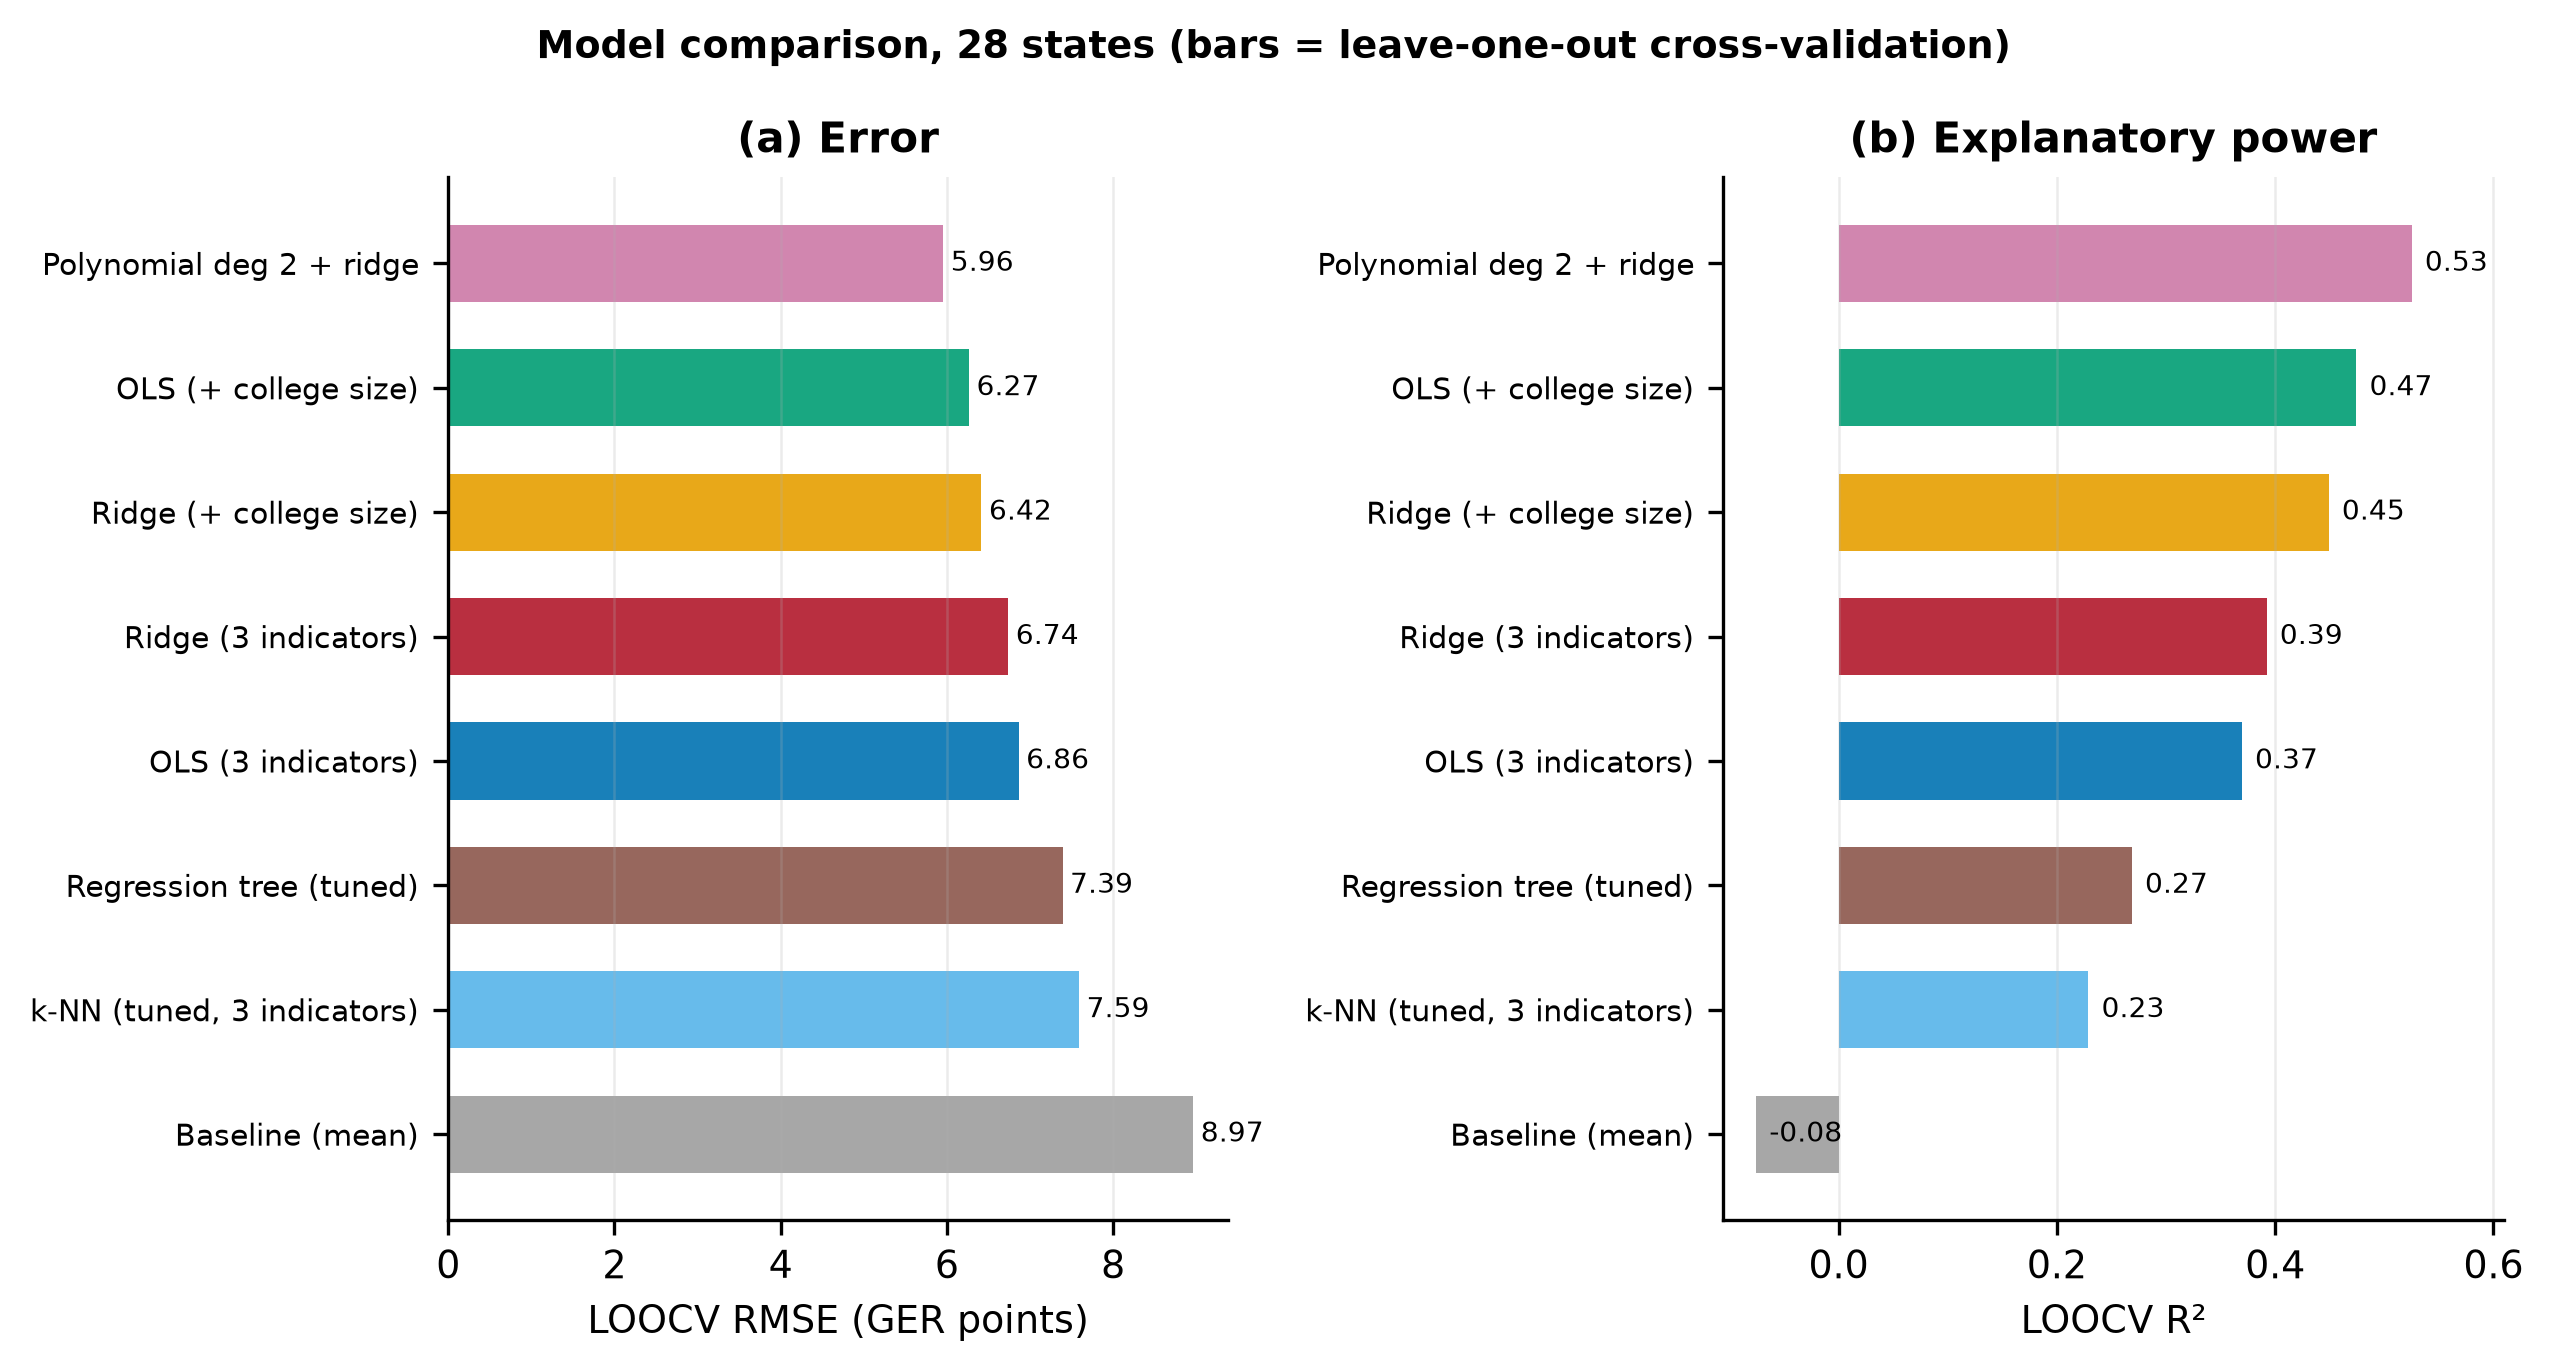
\includegraphics[width=\linewidth]{fig05_model_comparison.png}
\caption{LOOCV RMSE and \(R^2\) by model, 28 States. Lower RMSE and higher \(R^2\) are better. The polynomial ridge model is the best predictor; the tuned non-parametric models are worse than OLS out of sample. Source: \texttt{fig05\_model\_comparison.png}.}
\label{fig:modelcomp}
\end{figure}

\begin{figure}[htbp]
\centering
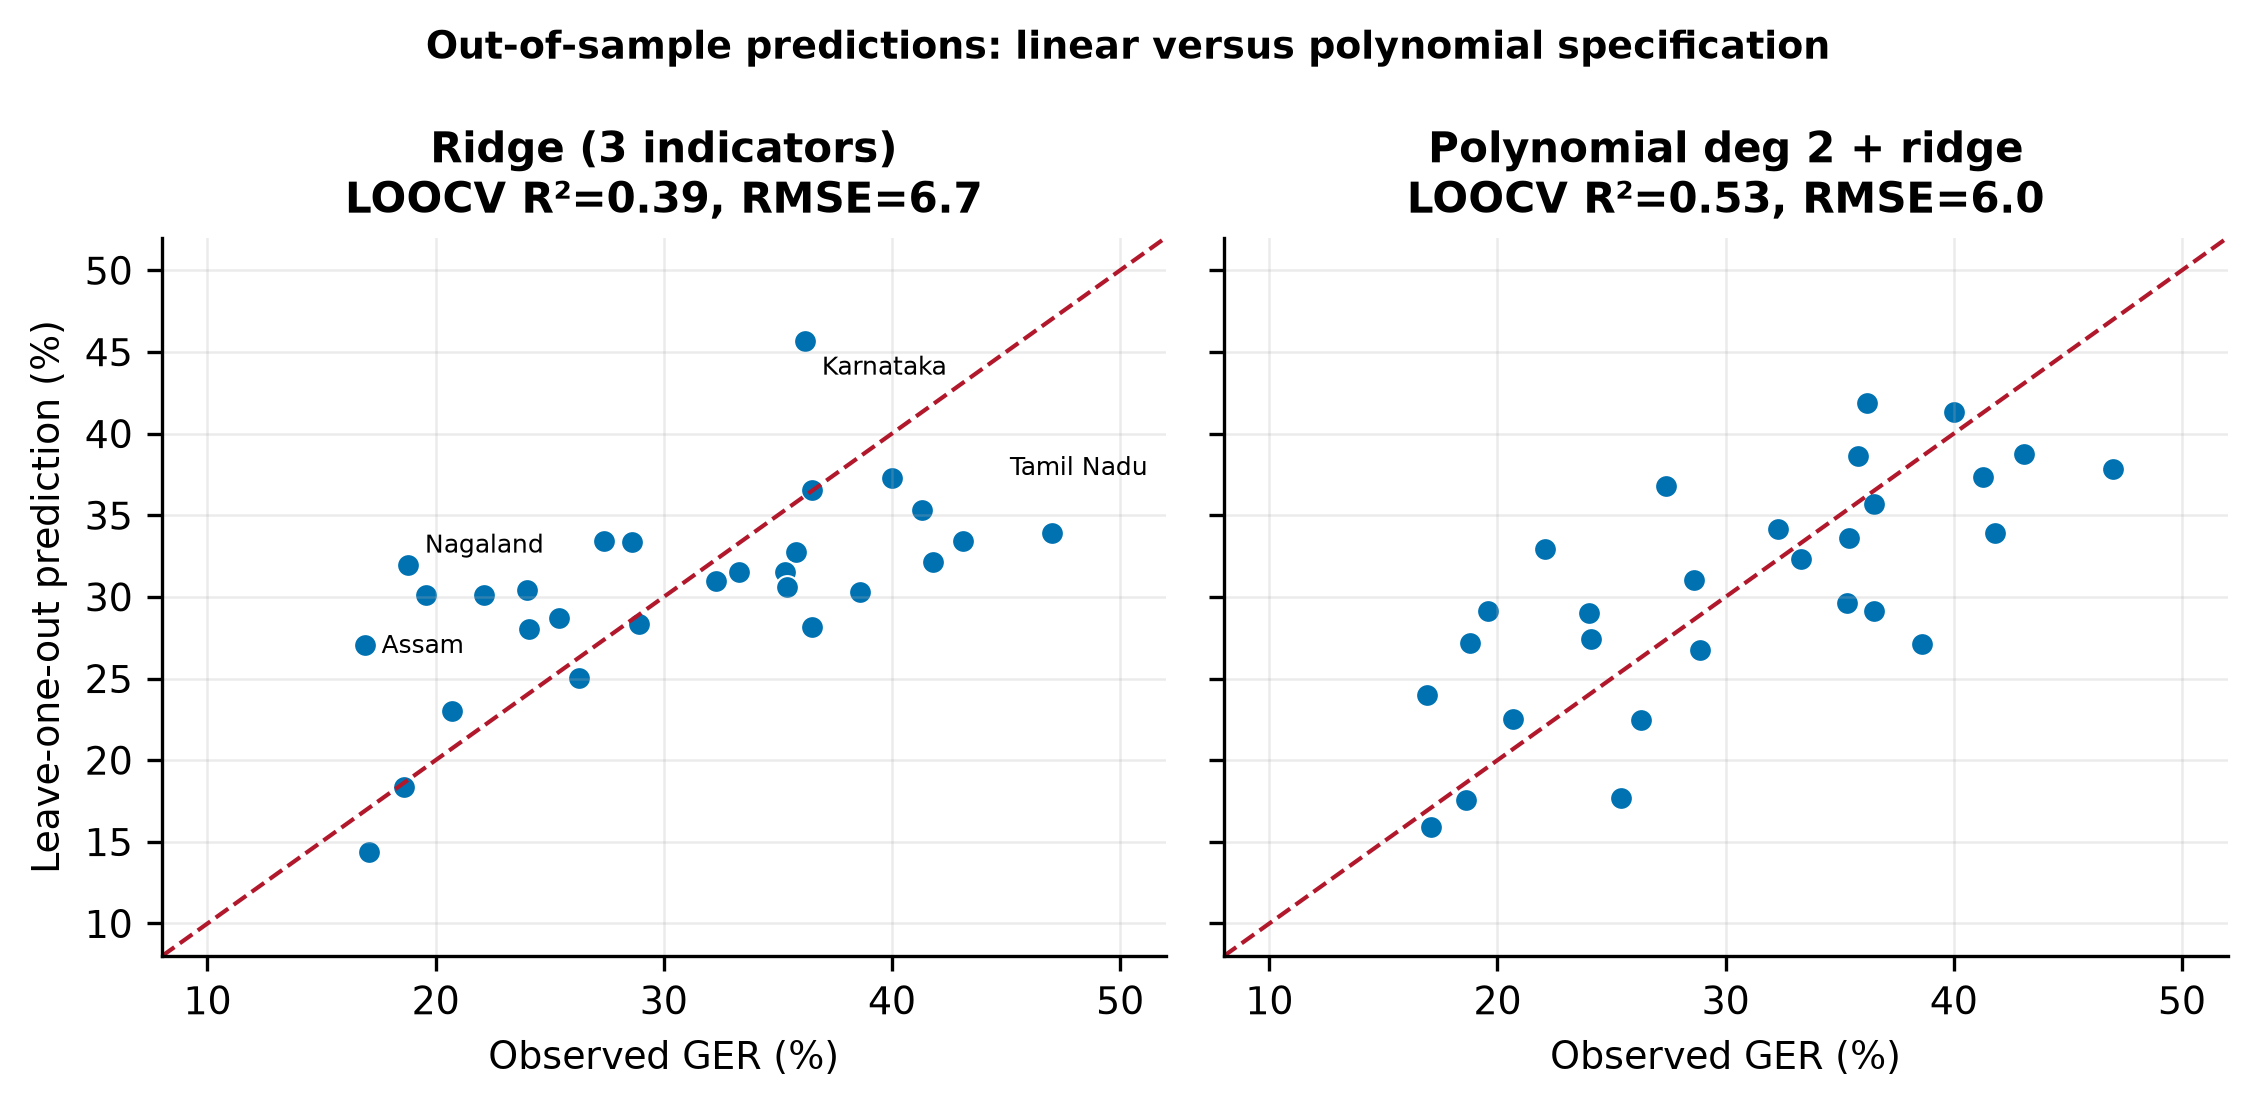
\includegraphics[width=\linewidth]{fig06_actual_vs_predicted.png}
\caption{Leave-one-out predictions against observed GER for ridge and polynomial ridge. The 45-degree line is perfect prediction. The polynomial tracks the middle of the distribution better but is less stable at the extremes. Source: \texttt{fig06\_actual\_vs\_predicted.png}.}
\label{fig:actualpred}
\end{figure}

Figure~\ref{fig:modelcomp} plots the two out-of-sample criteria, and Figure~\ref{fig:actualpred} shows that both models under-predict Tamil Nadu (47.0) and over-predict Karnataka (36.2), the two most influential States. The errors are not random: they reflect omitted variables such as private provision, urbanisation and demand, which are not in the three-indicator model.

\subsection{Coefficients and inference}

Table~\ref{tab:coefficients} reports the OLS coefficients with HC3 standard errors and bootstrap intervals. College density is the only coefficient that is statistically distinguishable from zero at conventional levels: \(+0.353\) GER points per additional college per lakh (HC3 SE 0.161; \(p = 0.029\); 95\% bootstrap interval 0.112 to 0.656). The standardised coefficient is 0.547, the largest in the model. Conditional on PTR and GPI, a one-standard-deviation increase in density is associated with about half a standard deviation of GER.

\begin{table}[htbp]
\centering
\caption{OLS coefficients, 28 States, 2021-22. HC3 standard errors; 95\% percentile bootstrap intervals from 2,000 resamples; standardised coefficients are SD of GER per SD of the predictor. Source: \texttt{table04\_coefficients.csv}.}
\label{tab:coefficients}
\resizebox{\textwidth}{!}{%
\begin{tabular}{@{}lrrrrrr@{}}
\toprule
Term & Coefficient & HC3 SE & \(p\)-value & Bootstrap 95\% CI & Standardised coefficient & VIF \\
\midrule
College density (\(\beta_D\)) & \textbf{0.353} & 0.161 & \textbf{0.029} & 0.112 to 0.656 & \textbf{0.547} & 1.78 \\
Pupil--teacher ratio (\(\beta_P\)) & $-0.189$ & 0.152 & 0.211 & $-0.637$ to 0.027 & $-0.247$ & 1.93 \\
Gender Parity Index (\(\beta_G\)) & 0.508 & 9.867 & 0.959 & $-22.46$ to 15.37 & 0.009 & 1.12 \\
\bottomrule
\end{tabular}}
\end{table}

The PTR coefficient is negative but imprecise: \(-0.189\) (\(p = 0.211\)), with a bootstrap interval that includes zero. More importantly, PTR is not exogenous. It is enrolment divided by teachers, so a State that expands enrolment without hiring teachers will mechanically show a higher PTR and a higher GER. The cross-sectional negative sign is therefore not a causal estimate of teacher quality. Section~\ref{sec:panel} shows that the sign flips in panel specifications.

The GPI coefficient is essentially zero and very imprecise: 0.508 (\(p = 0.959\)), with an interval from \(-22.5\) to 15.4. Conditional on college density and PTR, gender parity carries almost no independent information about the aggregate GER. This does not mean gender parity is unimportant. It means that the aggregate GER is not the right outcome for studying gender equity, and that most States are already close enough to parity that the remaining variation does not move the aggregate. Ten States remain below parity, and those gaps matter for female participation even when they do not shift the all-person GER.

\begin{figure}[htbp]
\centering
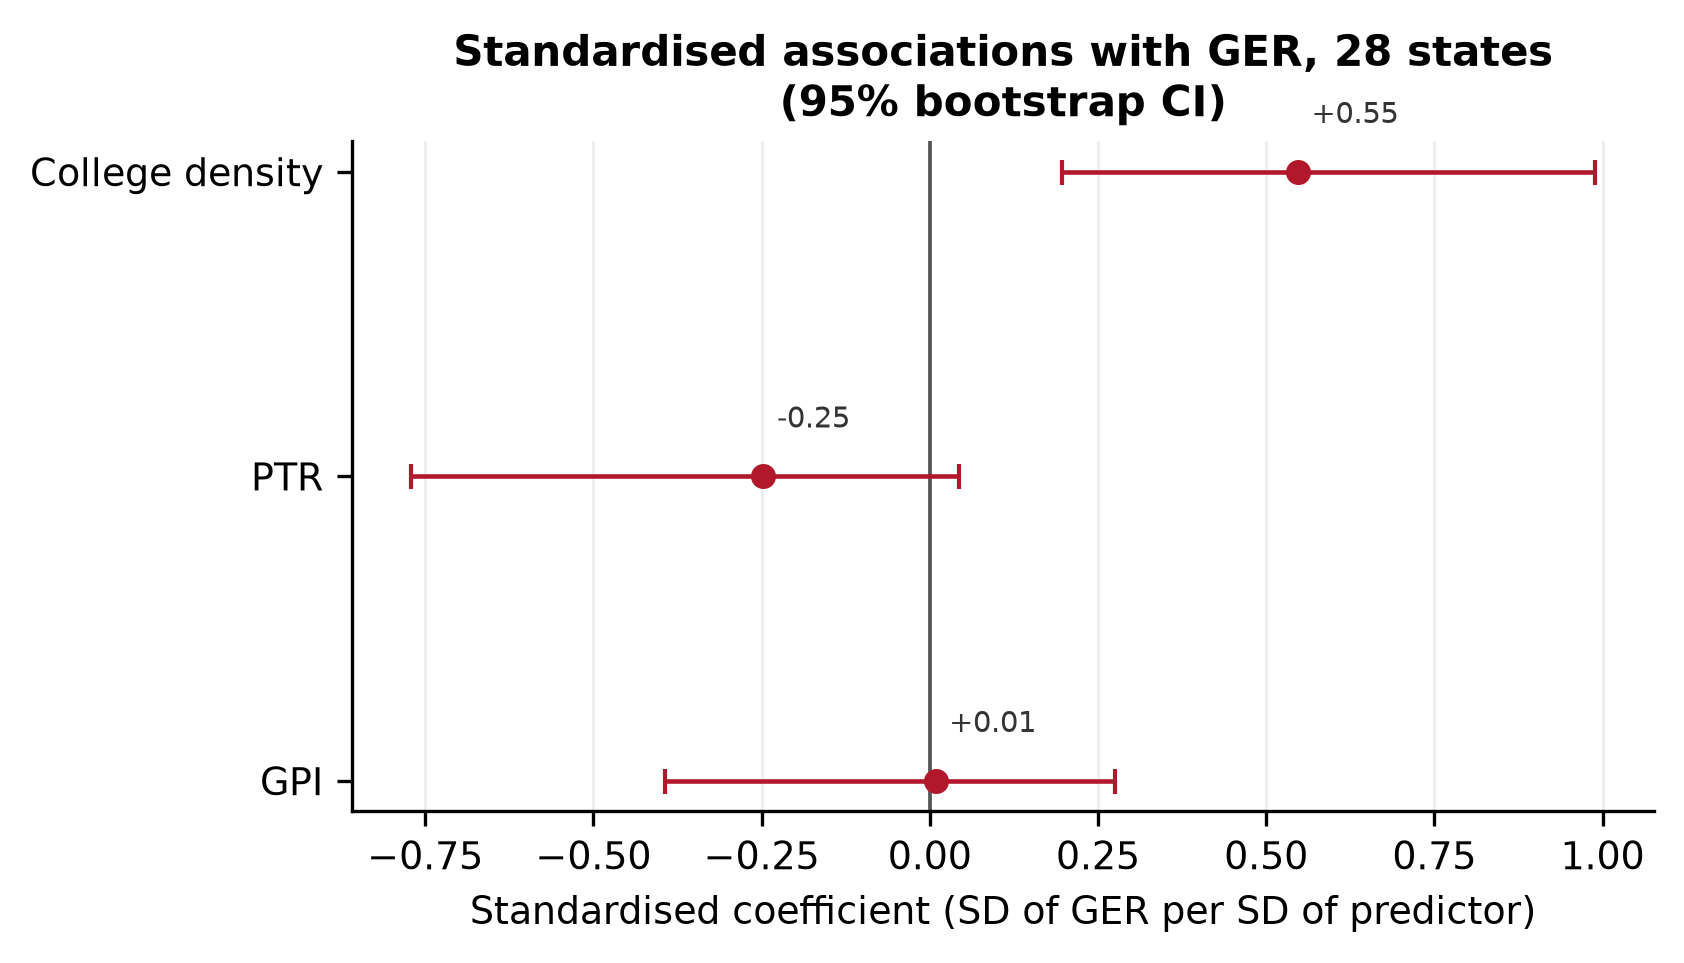
\includegraphics[width=0.9\linewidth]{fig08_coefficients.png}
\caption{Standardised coefficients with 95\% bootstrap confidence intervals, 28 States. Only college density has an interval that excludes zero. Source: \texttt{fig08\_coefficients.png}.}
\label{fig:coefplot}
\end{figure}

\begin{figure}[htbp]
\centering
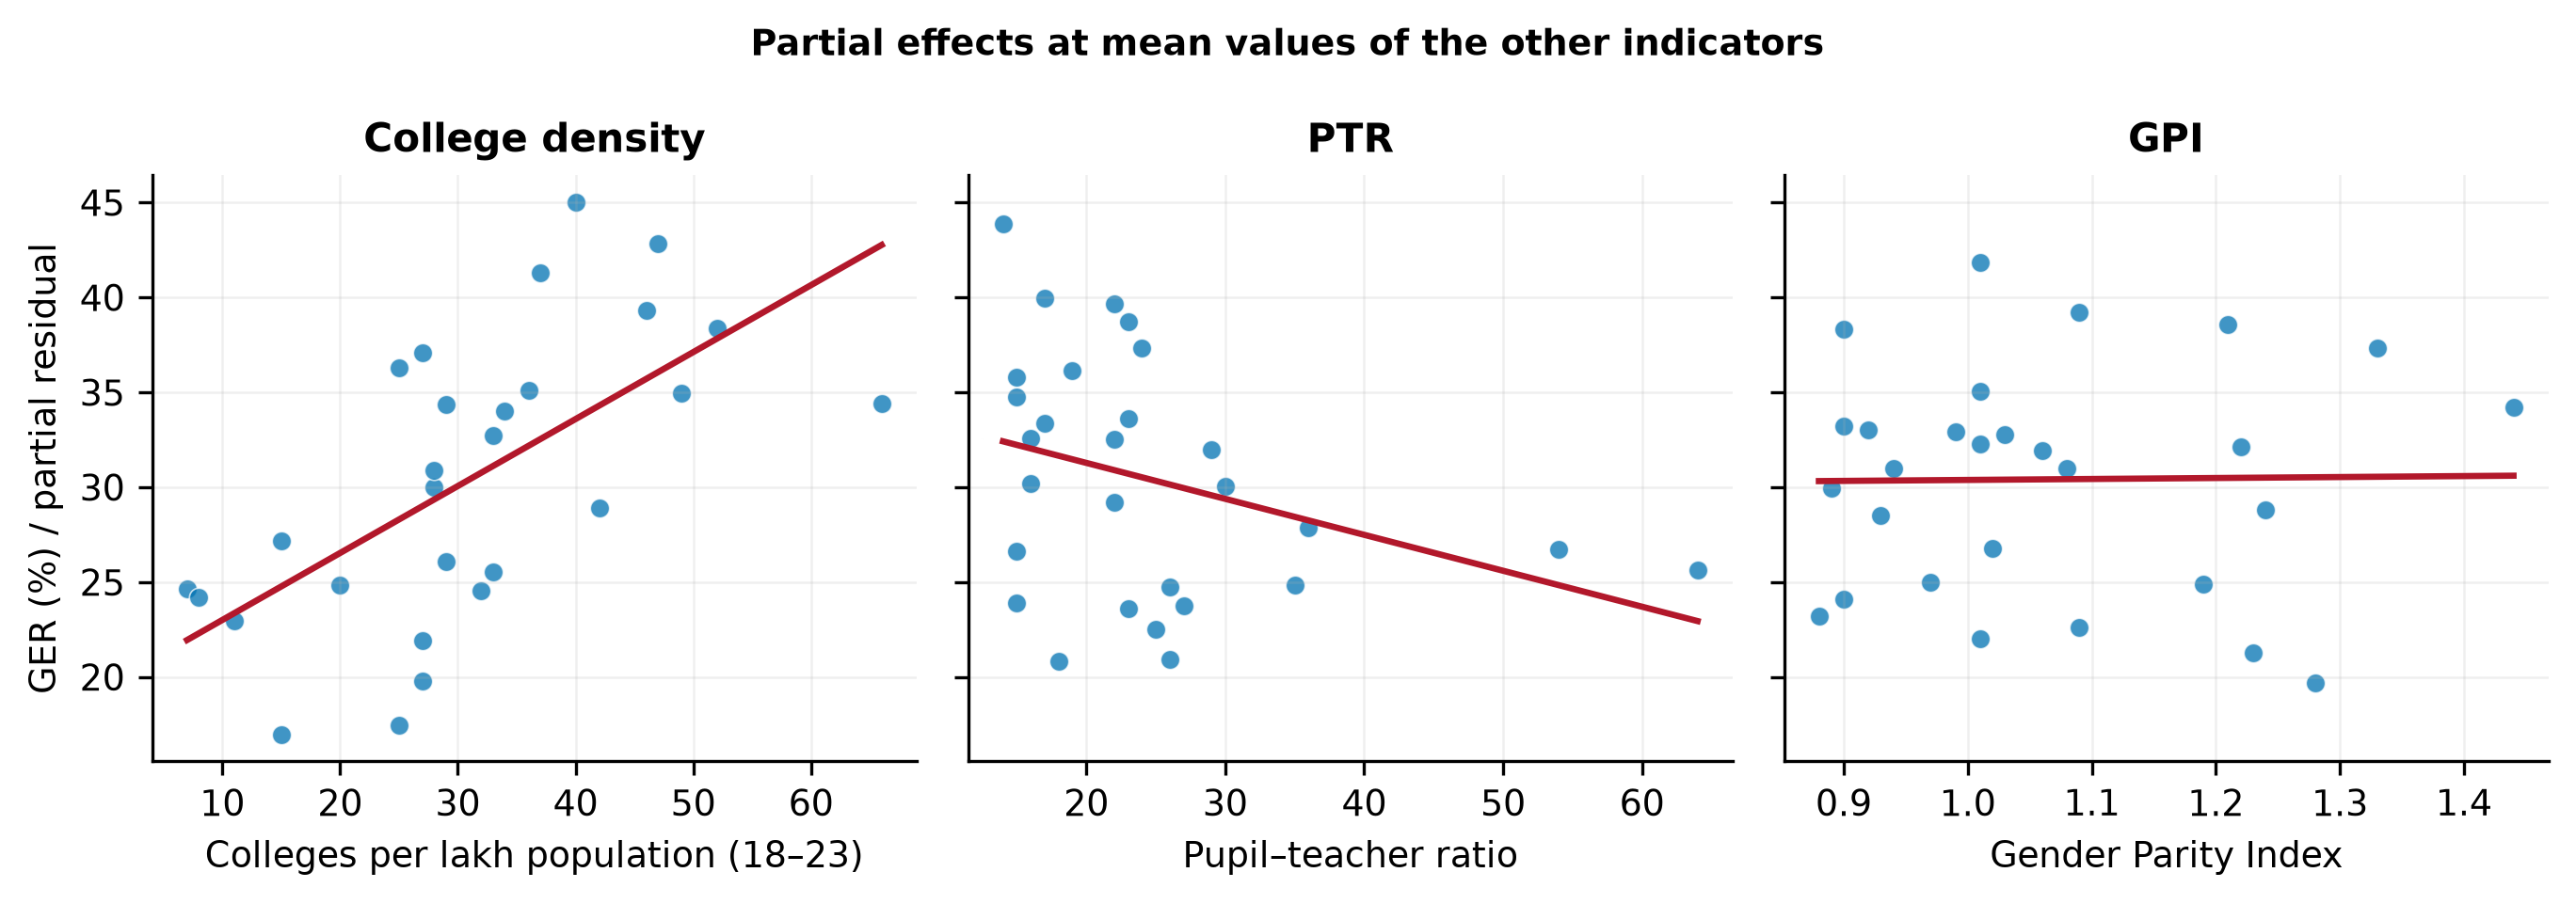
\includegraphics[width=\linewidth]{fig09_partial_effects.png}
\caption{Component-plus-residual partial effects at the mean of the other indicators, 28 States. The density slope is positive; the PTR slope is negative but imprecise; the GPI slope is almost flat. Source: \texttt{fig09\_partial\_effects.png}.}
\label{fig:partial}
\end{figure}

Figure~\ref{fig:coefplot} shows the bootstrap intervals graphically, and Figure~\ref{fig:partial} isolates each partial effect. The density slope is the only one that is clearly separated from zero; the PTR and GPI slopes are consistent with no effect once the other indicators are held constant.

\subsection{Diagnostics and influence}

The OLS residuals are consistent with the classical assumptions (Table~\ref{tab:diagnostics}). Shapiro--Wilk does not reject normality (\(W = 0.969\); \(p = 0.561\)), Breusch--Pagan does not reject homoskedasticity (LM \(= 3.05\); \(p = 0.384\)), and Ramsey RESET does not reject the linear functional form (\(F = 0.021\); \(p = 0.885\)). The condition number is 489, which is moderate for a model with three correlated predictors. No State has a studentised residual above 2 in absolute value.

\begin{table}[htbp]
\centering
\scriptsize
\setlength{\tabcolsep}{3pt}
\caption{Residual diagnostics and influence, OLS three-indicator model, 28 States. The Cook's distance threshold is \(4/n = 0.143\). Source: \texttt{table05\_diagnostics.csv}.}
\label{tab:diagnostics}
\begin{tabular}{@{}p{4.5cm}rp{1.6cm}p{4.1cm}@{}}
\toprule
Diagnostic & Statistic & \(p\)-value & Interpretation \\
\midrule
Shapiro--Wilk (normality) & \(W = 0.969\) & 0.561 & No evidence of non-normality \\
Breusch--Pagan (heterosked.) & LM \(= 3.05\) & 0.384 & No evidence of heteroskedasticity \\
Ramsey RESET (functional form) & \(F = 0.021\) & 0.885 & No evidence of missed nonlinearity \\
Condition number & 489 & --- & Moderate collinearity \\
Maximum Cook's distance & 0.338 & --- & Karnataka; threshold \(4/n = 0.143\) \\
Influential States (Cook's \(D > 4/n\)) & 2 & --- & Karnataka, Nagaland \\
Studentised residuals \(> 2\) in \(|\cdot|\) & 0 & --- & No severe outliers \\
\bottomrule
\end{tabular}
\end{table}

Figure~\ref{fig:residuals} shows the four residual plots; none suggests a systematic departure from the linear specification. Two States are influential. Karnataka has Cook's distance 0.338 and leverage 0.338: it is the highest-density State (66 colleges per lakh) but has a lower GER than the model predicts (residual \(-8.35\)). Nagaland has Cook's distance 0.156 and the largest negative residual (\(-10.85\)). Tamil Nadu has the largest positive residual (\(+11.43\)) but low leverage, so its influence is smaller (Cook's \(D = 0.083\)). Figure~\ref{fig:influence} plots the influence measures, and Figure~\ref{fig:poly} shows the out-of-range behaviour that rules out the polynomial for projection.

\begin{figure}[htbp]
\centering
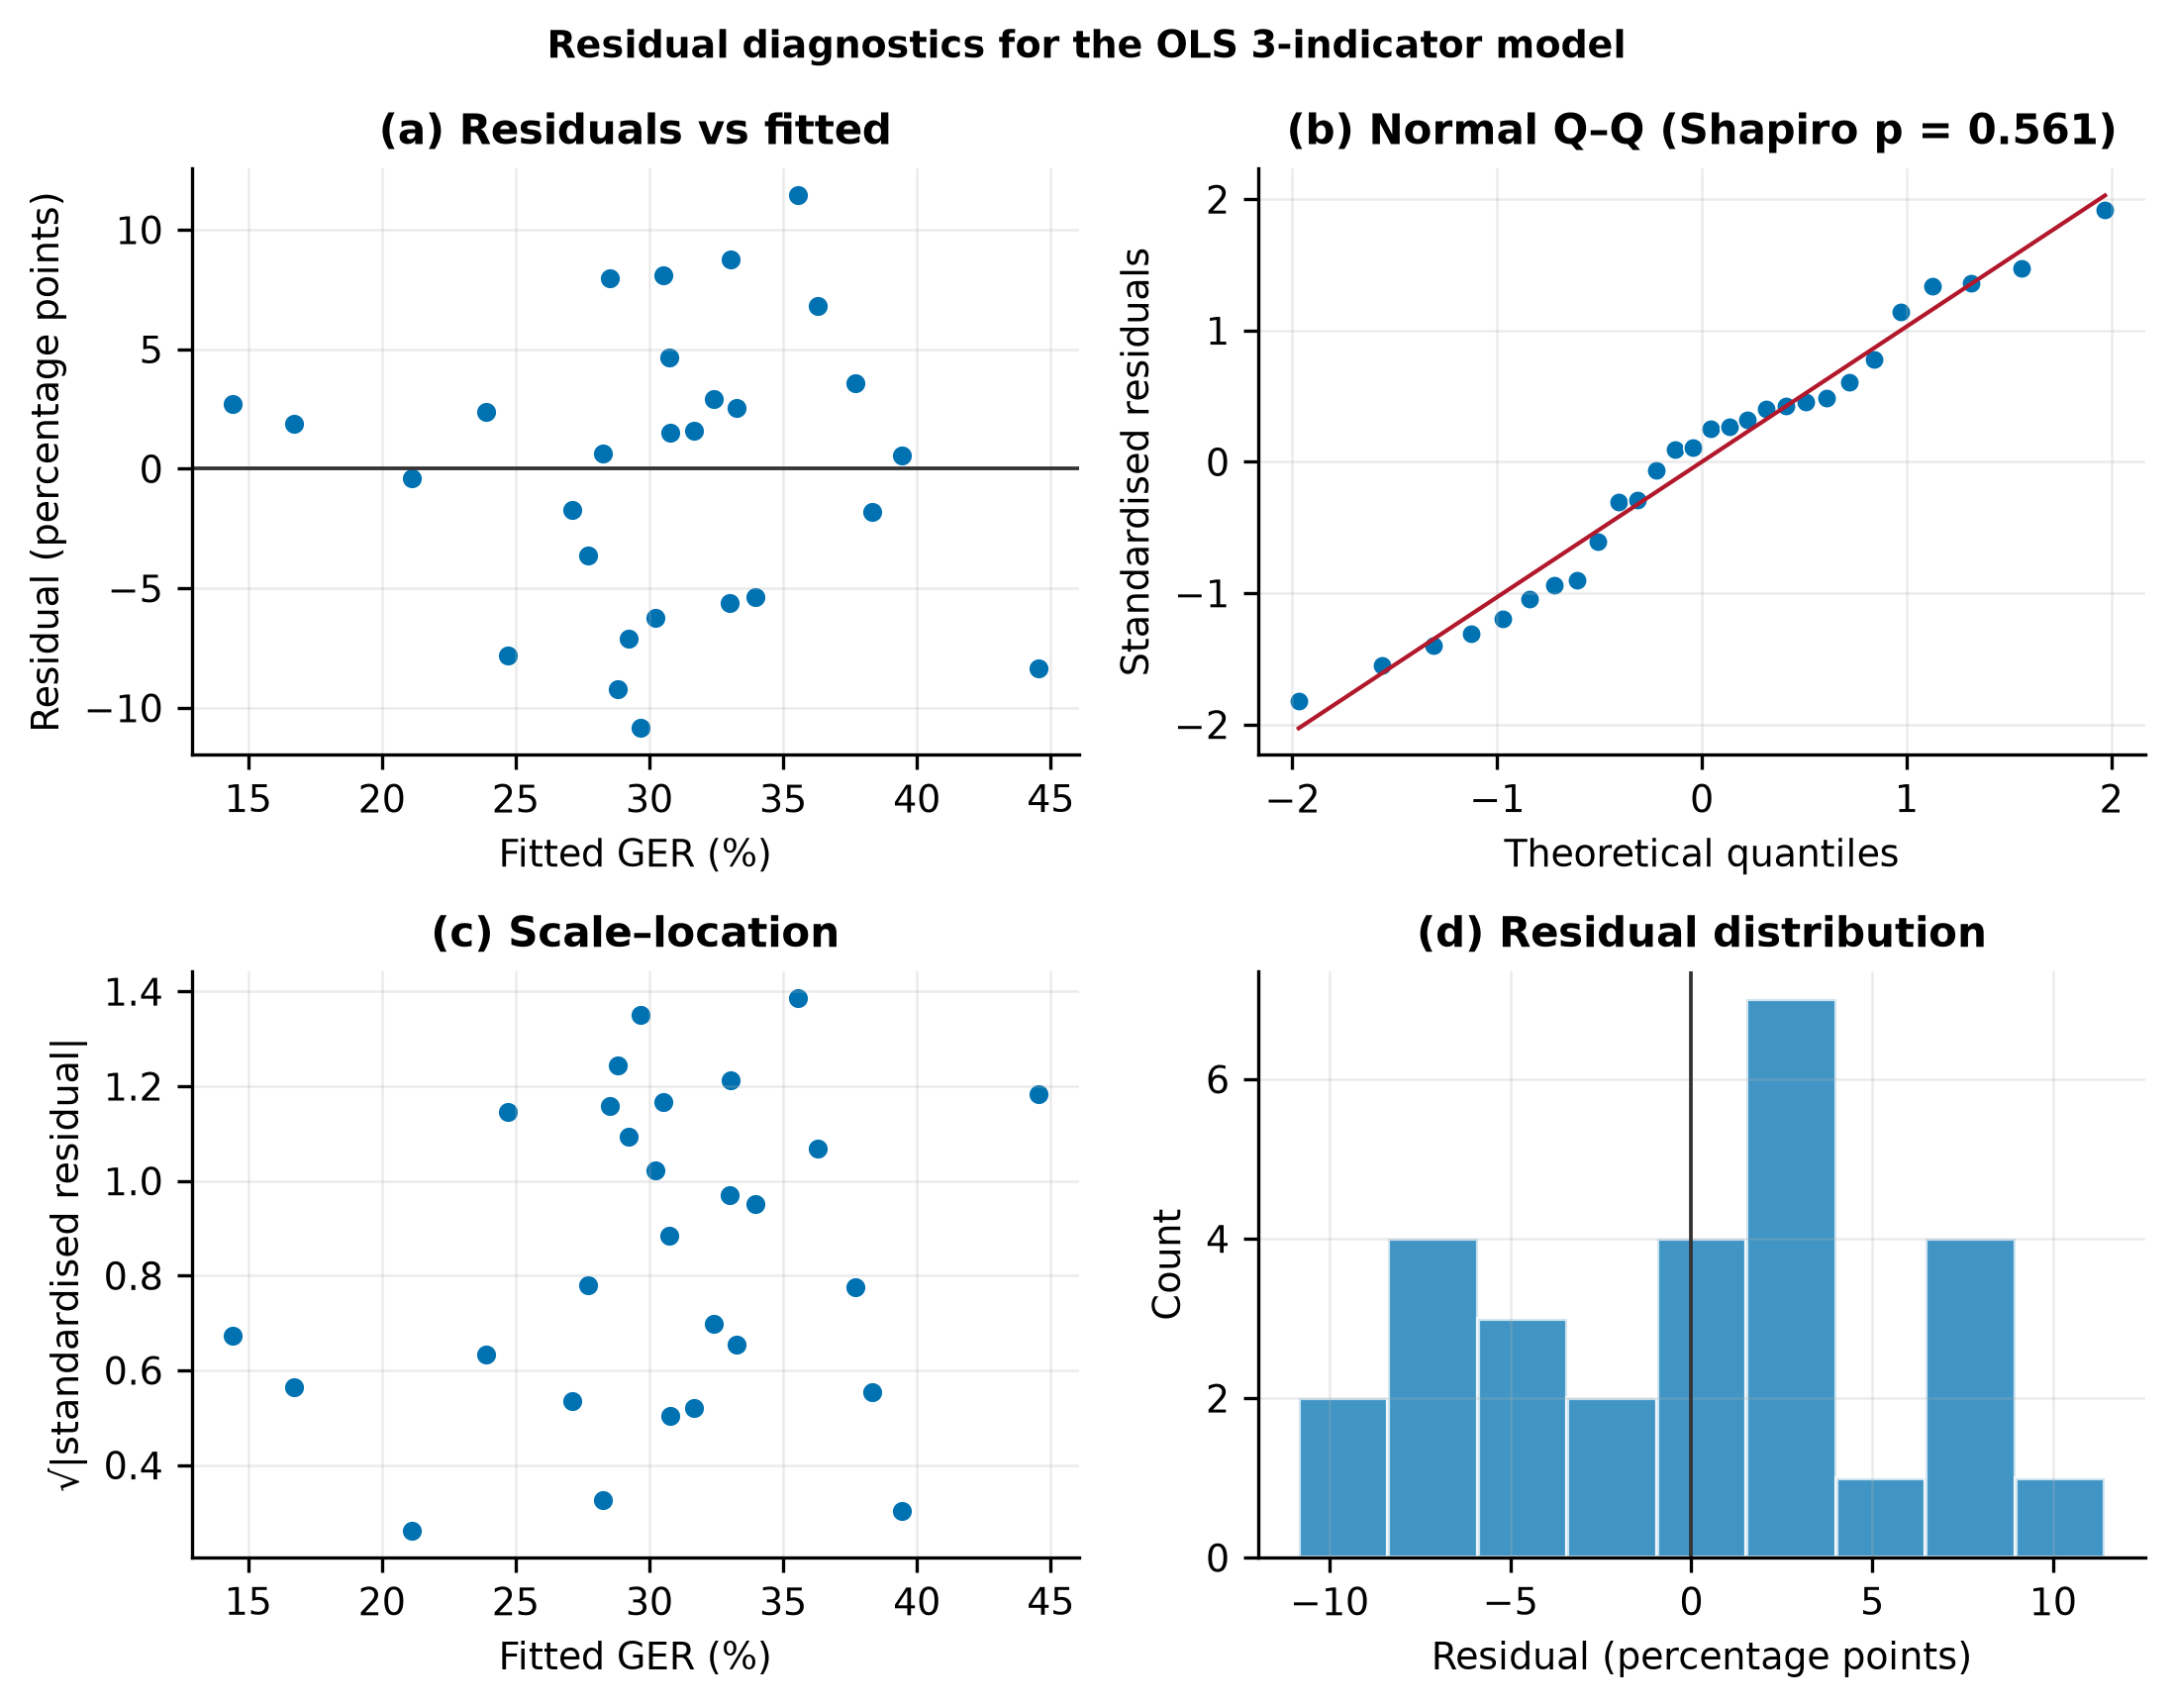
\includegraphics[width=\linewidth]{fig07_residual_diagnostics.png}
\caption{Residual diagnostics for the OLS three-indicator model: residuals versus fitted values, normal Q--Q plot, scale--location plot and residual histogram. Source: \texttt{fig07\_residual\_diagnostics.png}.}
\label{fig:residuals}
\end{figure}

\begin{figure}[htbp]
\centering
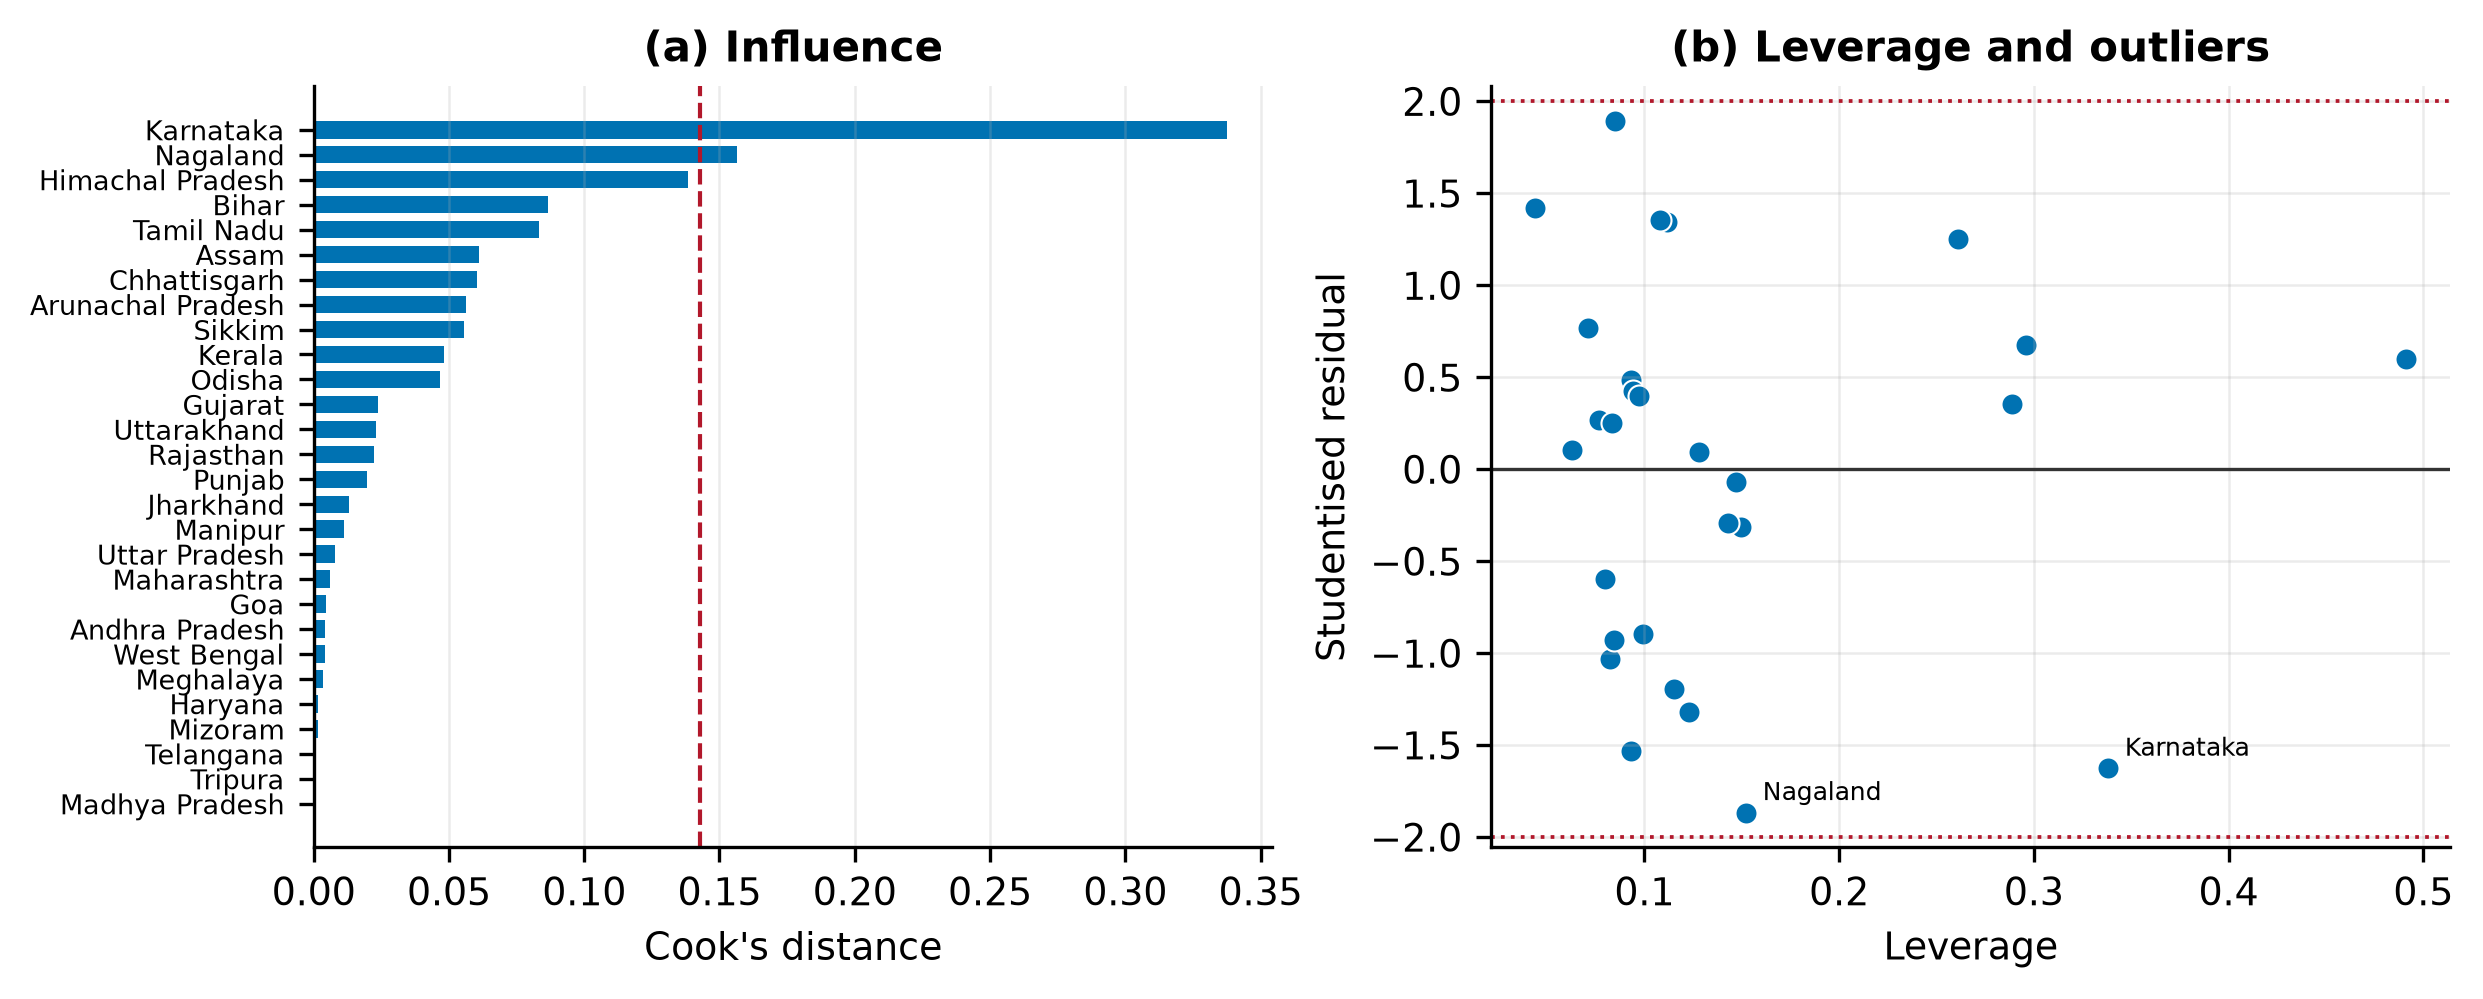
\includegraphics[width=\linewidth]{fig10_influence.png}
\caption{Influence diagnostics: Cook's distance by State and leverage against studentised residual, 28 States. Karnataka and Nagaland exceed the \(4/n\) threshold. Source: \texttt{fig10\_influence.png}.}
\label{fig:influence}
\end{figure}

\begin{figure}[htbp]
\centering
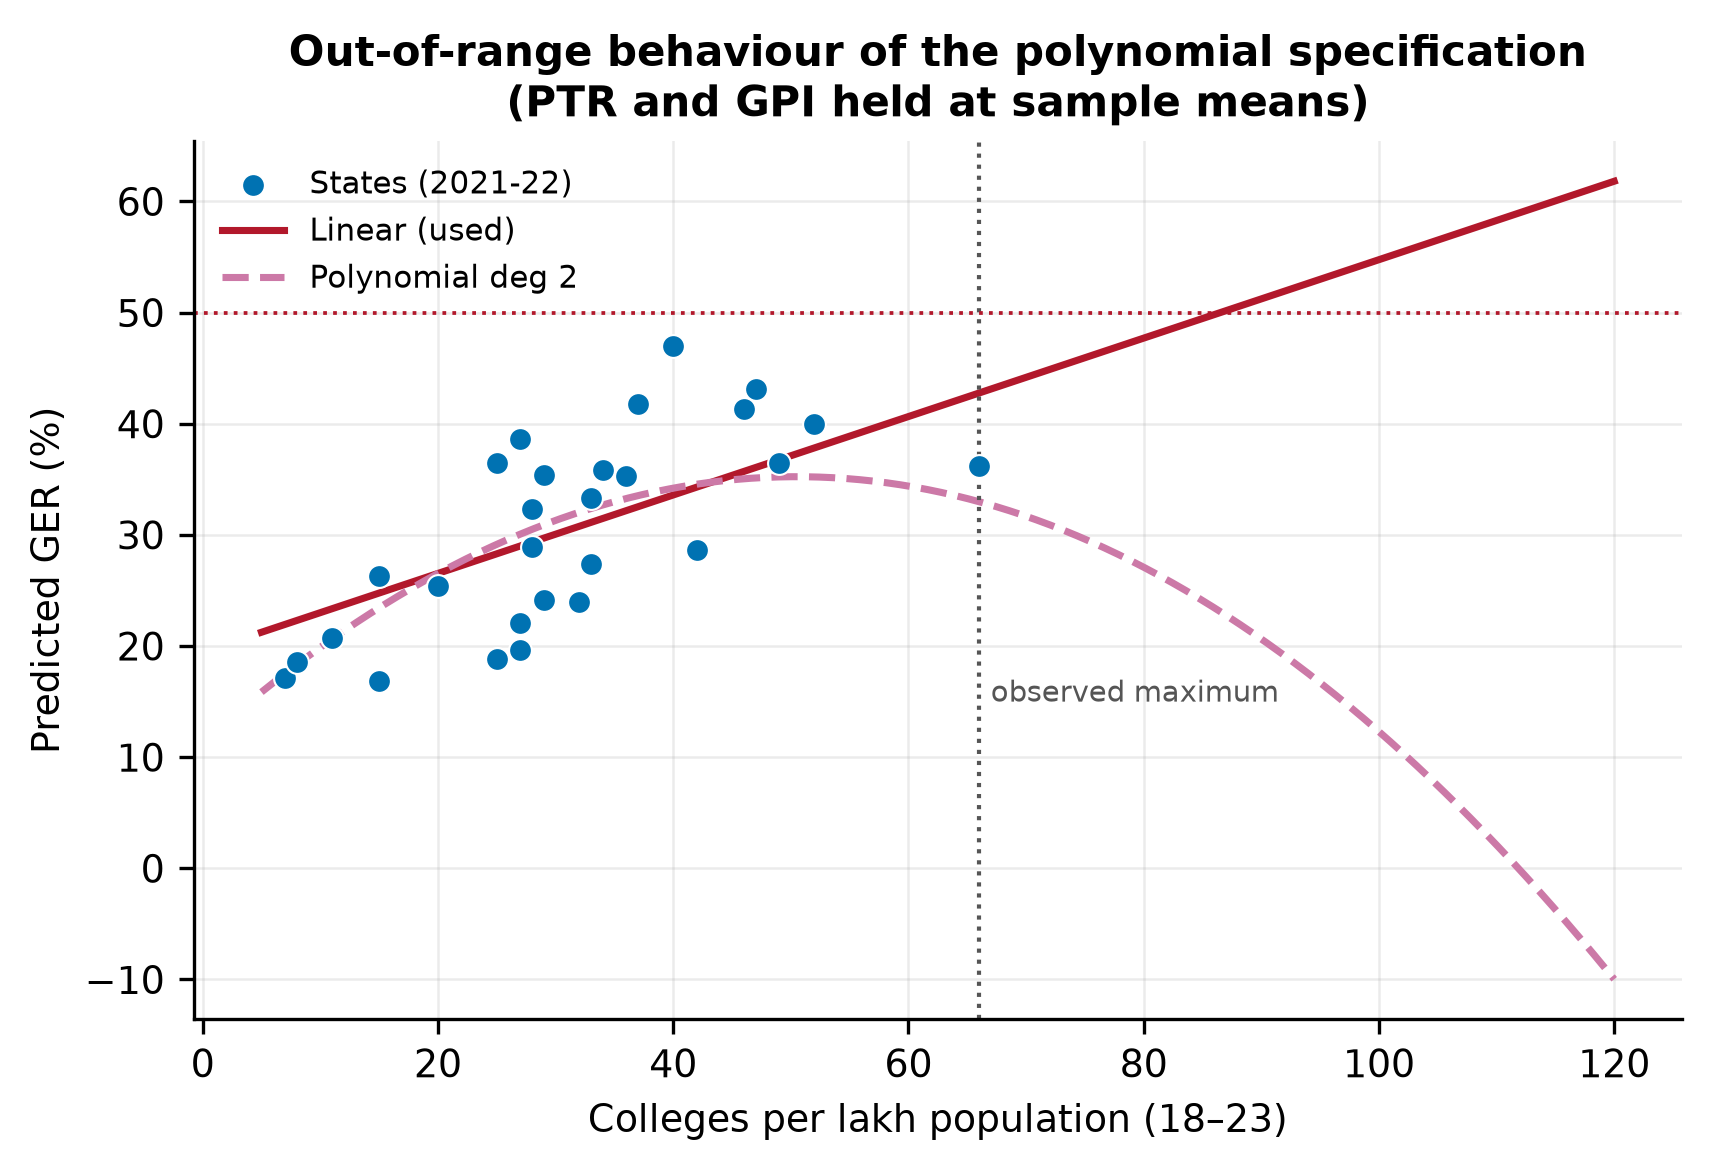
\includegraphics[width=0.9\linewidth]{fig11_polynomial_instability.png}
\caption{Out-of-range behaviour of the polynomial specification. The degree-2 fit turns downward beyond the observed density range and eventually predicts negative GER, whereas the linear fit remains monotone. This is why the polynomial is a predictive benchmark, not the projection model. Source: \texttt{fig11\_polynomial\_instability.png}.}
\label{fig:poly}
\end{figure}

\subsection{Panel and sensitivity checks}\label{sec:panel}

Table~\ref{tab:sensitivity} reports the panel and leave-out checks. The density association is stable: 0.355 with year fixed effects, 0.398 with State and year fixed effects, and 0.752 in first differences. The first-difference estimate is larger, which suggests that within-State expansion is associated with larger GER gains than the cross-section alone implies. The short panel and measurement error caution against over-interpretation, but the sign and order of magnitude are consistent.

\begin{table}[htbp]
\centering
\caption{Panel, leave-out and UT-inclusive specifications. Panel rows use State-clustered standard errors; cross-section HC3 \(p\)-values are reported in Table~\ref{tab:coefficients}. The Sikkim-excluded row checks whether the common trend depends on one anomalous series. Source: \texttt{table07\_sensitivity.csv}.}
\label{tab:sensitivity}
\resizebox{\textwidth}{!}{%
\begin{tabular}{@{}lrrrrr@{}}
\toprule
Specification & \(n\) & Density coef. & PTR coef. & GPI coef. & \(R^2\) / LOOCV \(R^2\) \\
\midrule
Cross-section OLS & 28 & 0.353 & $-0.189$ & 0.508 & \(R^2 = 0.543\) \\
Panel, year FE & 140 & 0.355 & $-0.215$ & $-0.846$ & \(R^2 = 0.480\) \\
Panel, year FE excluding Sikkim & 135 & 0.416 & $-0.107$ & $+2.287$ & \(R^2 = 0.585\) \\
Panel, State + year FE & 140 & 0.398 & $+0.343$ & $-26.98$ & \(R^2 = 0.945\) \\
First differences & 112 & 0.752 & $+0.146$ & $-28.39$ & \(R^2 = 0.395\) \\
OLS excluding Karnataka & 27 & 0.474 & $-0.136$ & $-1.245$ & \(R^2 = 0.586\); LOOCV \(R^2 = 0.457\) \\
OLS excluding Karnataka + Bihar & 26 & 0.461 & $-0.208$ & $-1.564$ & \(R^2 = 0.555\); LOOCV \(R^2 = 0.392\) \\
All 35 units, core & 35 & --- & --- & --- & LOOCV \(R^2 = 0.158\) \\
All 35 units, core + UT dummy & 35 & --- & --- & --- & LOOCV \(R^2 = 0.180\) \\
\bottomrule
\end{tabular}}
\end{table}

PTR is not robust. It is \(-0.215\) in the year fixed-effects model but \(+0.343\) with State fixed effects and \(+0.146\) in first differences. The sign flip is exactly what one would expect from reverse causality and from the mechanical relationship between PTR and enrolment. A State that expands enrolment without matching teacher hiring will raise its PTR; a State that hires teachers without expanding enrolment will lower it. The cross-sectional negative correlation is therefore not a credible estimate of the effect of teacher supply.

GPI is also unstable and imprecisely estimated. The large negative coefficients in the State fixed-effects and first-difference models reflect limited within-State variation and collinearity, not a credible policy effect. The aggregate GER is simply not a good outcome for identifying gender-specific constraints.

The common annual trend from the year fixed-effects model is 0.866 GER points per year (SE 0.174). Over 14 years this is about 12.1 points, with a 95\% interval of roughly 7.2 to 17.0 points. This trend is a key input to the projection and a major source of uncertainty. It is an average from a short, Covid-affected panel; it may not continue for 14 years, and it is unlikely to be the same in every State.

One series needs a caveat. Sikkim reports a GER of 66.9\% in 2019-20, having reported 48.1\% the year before and 39.9\% the year after. A 27-point fall in one year is not a plausible change in participation; it is almost certainly a change in how the State reported enrolment or population. Sikkim is retained in the primary estimates because deleting a State for looking unusual is a judgement that should be made transparently rather than silently, and because the alternative would be to drop a genuine data point. As a check, the year fixed-effects model is re-estimated without Sikkim: the density coefficient rises to 0.416, the common trend falls only to 0.845 (SE 0.161), and \(R^2\) rises from 0.480 to 0.585. The trend used in the projection, 0.866, is therefore not an artefact of the Sikkim series, and the density result is, if anything, stronger without it. Figure~\ref{fig:trajectories} annotates the observation.

The leave-out checks strengthen the density result. Excluding Karnataka raises the density coefficient to 0.474 (\(p = 0.001\)) and the in-sample \(R^2\) to 0.586. Excluding Karnataka and Bihar gives 0.461 (\(p = 0.002\)) and \(R^2 = 0.555\). The coefficient is larger without Karnataka because Karnataka is a high-density, low-GER outlier that pulls the slope down. The result does not depend on one or two States.

The UT-inclusive models perform much worse out of sample: LOOCV \(R^2\) is 0.158 without a UT dummy and 0.180 with one, and RMSE is about 11.2--11.4. This confirms that UTs are not exchangeable with States and justifies the primary sample choice.

\subsection{Projections to 2035-36}

Table~\ref{tab:scenariosummary} summarises the three scenarios. Under the reference scenario (S2), 13 of 28 States reach 50\% by 2035-36. Under the damped scenario (S1), only three do. The reform scenario (S3) also produces 13 crossings: PTR and GPI reforms raise the mean projection by about 1.2 points, but they do not move any additional State across the line.

\begin{table}[htbp]
\centering
\caption{Scenario summary, 28 States, 2035-36. Point estimates and probabilities come from 2,000 bootstrap draws; the last column counts States by \(P(\GER \ge 50\%)\) as on track / at risk / off track. State detail is in \texttt{table06\_projections\_2035.csv}. Source: \texttt{table09\_scenario\_summary.csv}.}
\label{tab:scenariosummary}
\resizebox{\textwidth}{!}{%
\begin{tabular}{@{}lrrrrrrl@{}}
\toprule
Scenario & Point \(\ge 50\%\) & \(P(\GER \ge 50\%) \ge 0.5\) & Mean & Median & Min & Max & On / at risk / off \\
\midrule
S1 Damped & 3 & 3 & 38.2 & 40.7 & 23.2 & 56.2 & 3 / 6 / 19 \\
S2 Recent trend (reference) & 13 & 13 & 45.8 & 49.5 & 28.5 & 65.3 & 13 / 3 / 12 \\
S3 NEP reform & 13 & 13 & 47.0 & 49.7 & 28.5 & 65.3 & 13 / 4 / 11 \\
\bottomrule
\end{tabular}}
\end{table}

The 13 States reaching 50\% under S2 are Tamil Nadu (65.3), Himachal Pradesh (57.7), Uttarakhand (53.9), Kerala (55.9), Telangana (53.4), Sikkim (56.9), Arunachal Pradesh (56.0), Karnataka (60.3), Goa (50.4), Manipur (51.2), Maharashtra (51.1), Mizoram (50.6) and Rajasthan (51.8). Three are at risk rather than off track: Andhra Pradesh (49.9; \(P = 0.49\)), Haryana (49.1; \(P = 0.47\)) and Madhya Pradesh (46.0; \(P = 0.29\)). The remaining 12 are off track: Punjab (39.5), West Bengal (42.1), Meghalaya (40.0), Uttar Pradesh (37.5), Gujarat (38.6), Odisha (39.2), Tripura (31.6), Chhattisgarh (35.4), Nagaland (28.5), Jharkhand (30.7), Bihar (29.2) and Assam (30.3).

\begin{figure}[htbp]
\centering
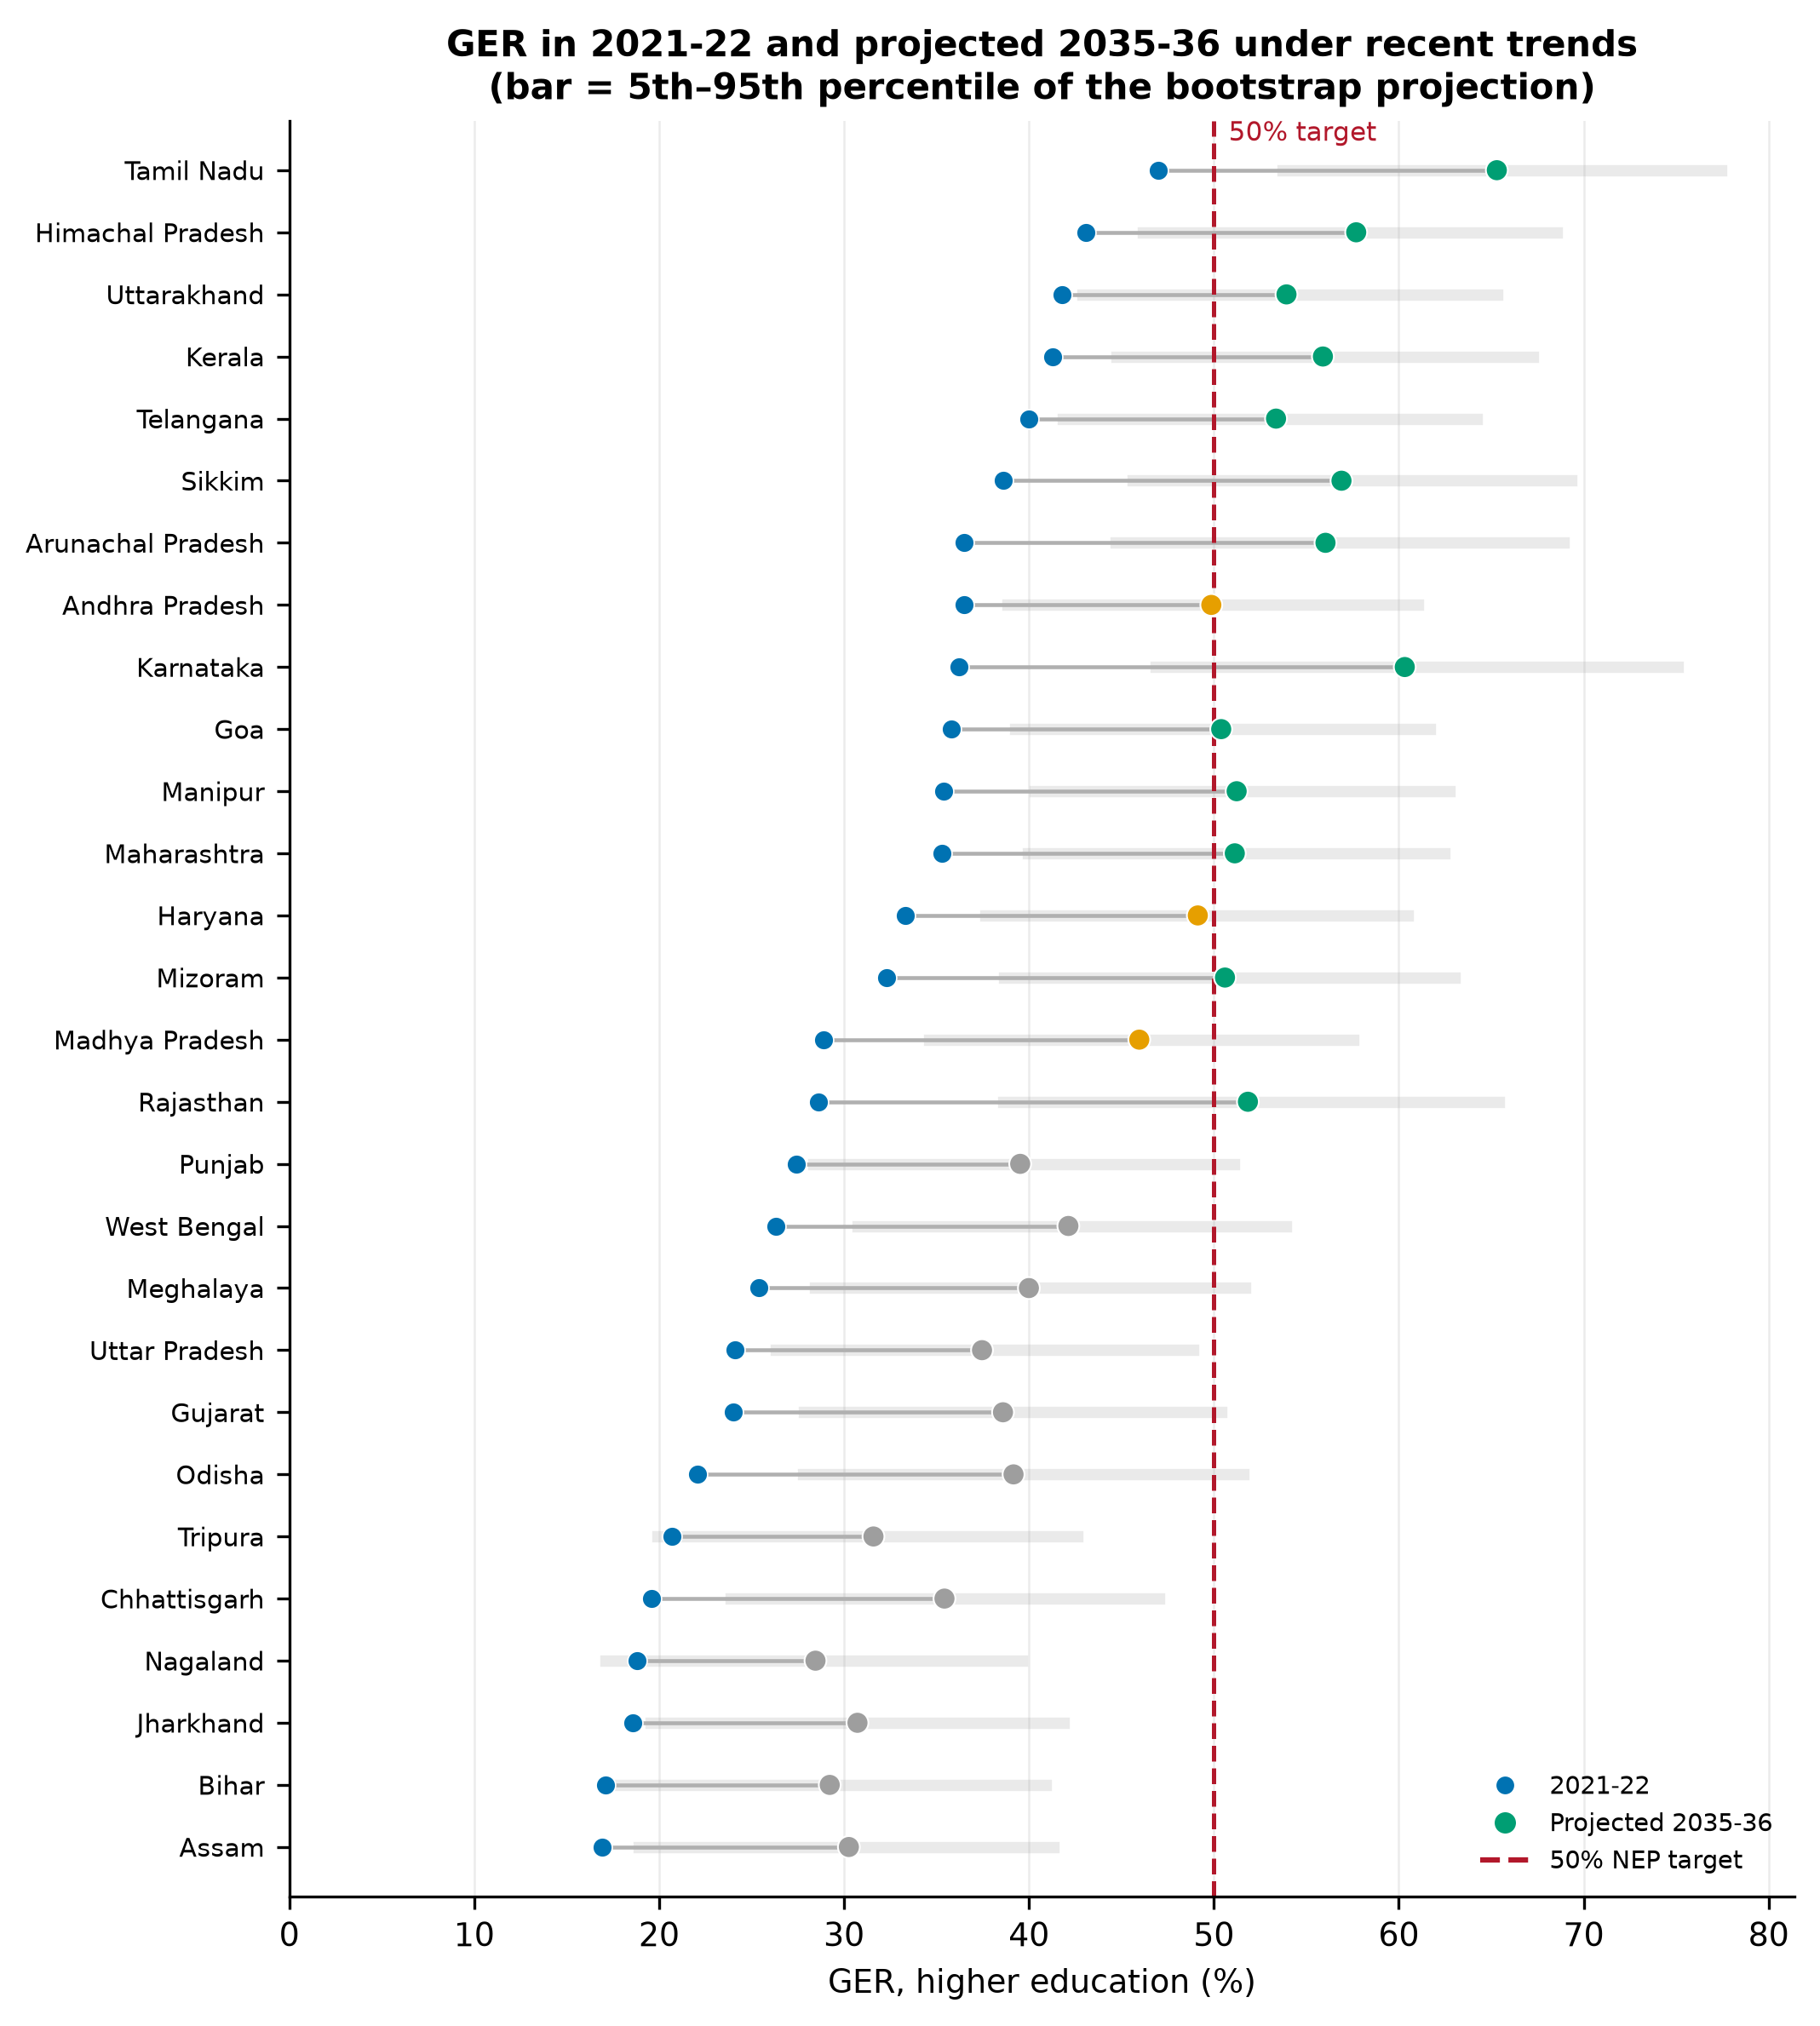
\includegraphics[width=\linewidth]{fig12_projection_dumbbell.png}
\caption{Observed GER in 2021-22 and projected GER in 2035-36 under recent trends, 28 States. Bars show the 5th--95th percentile bootstrap interval; the dashed line is the 50\% target. Source: \texttt{fig12\_projection\_dumbbell.png}.}
\label{fig:dumbbell}
\end{figure}

\begin{figure}[htbp]
\centering
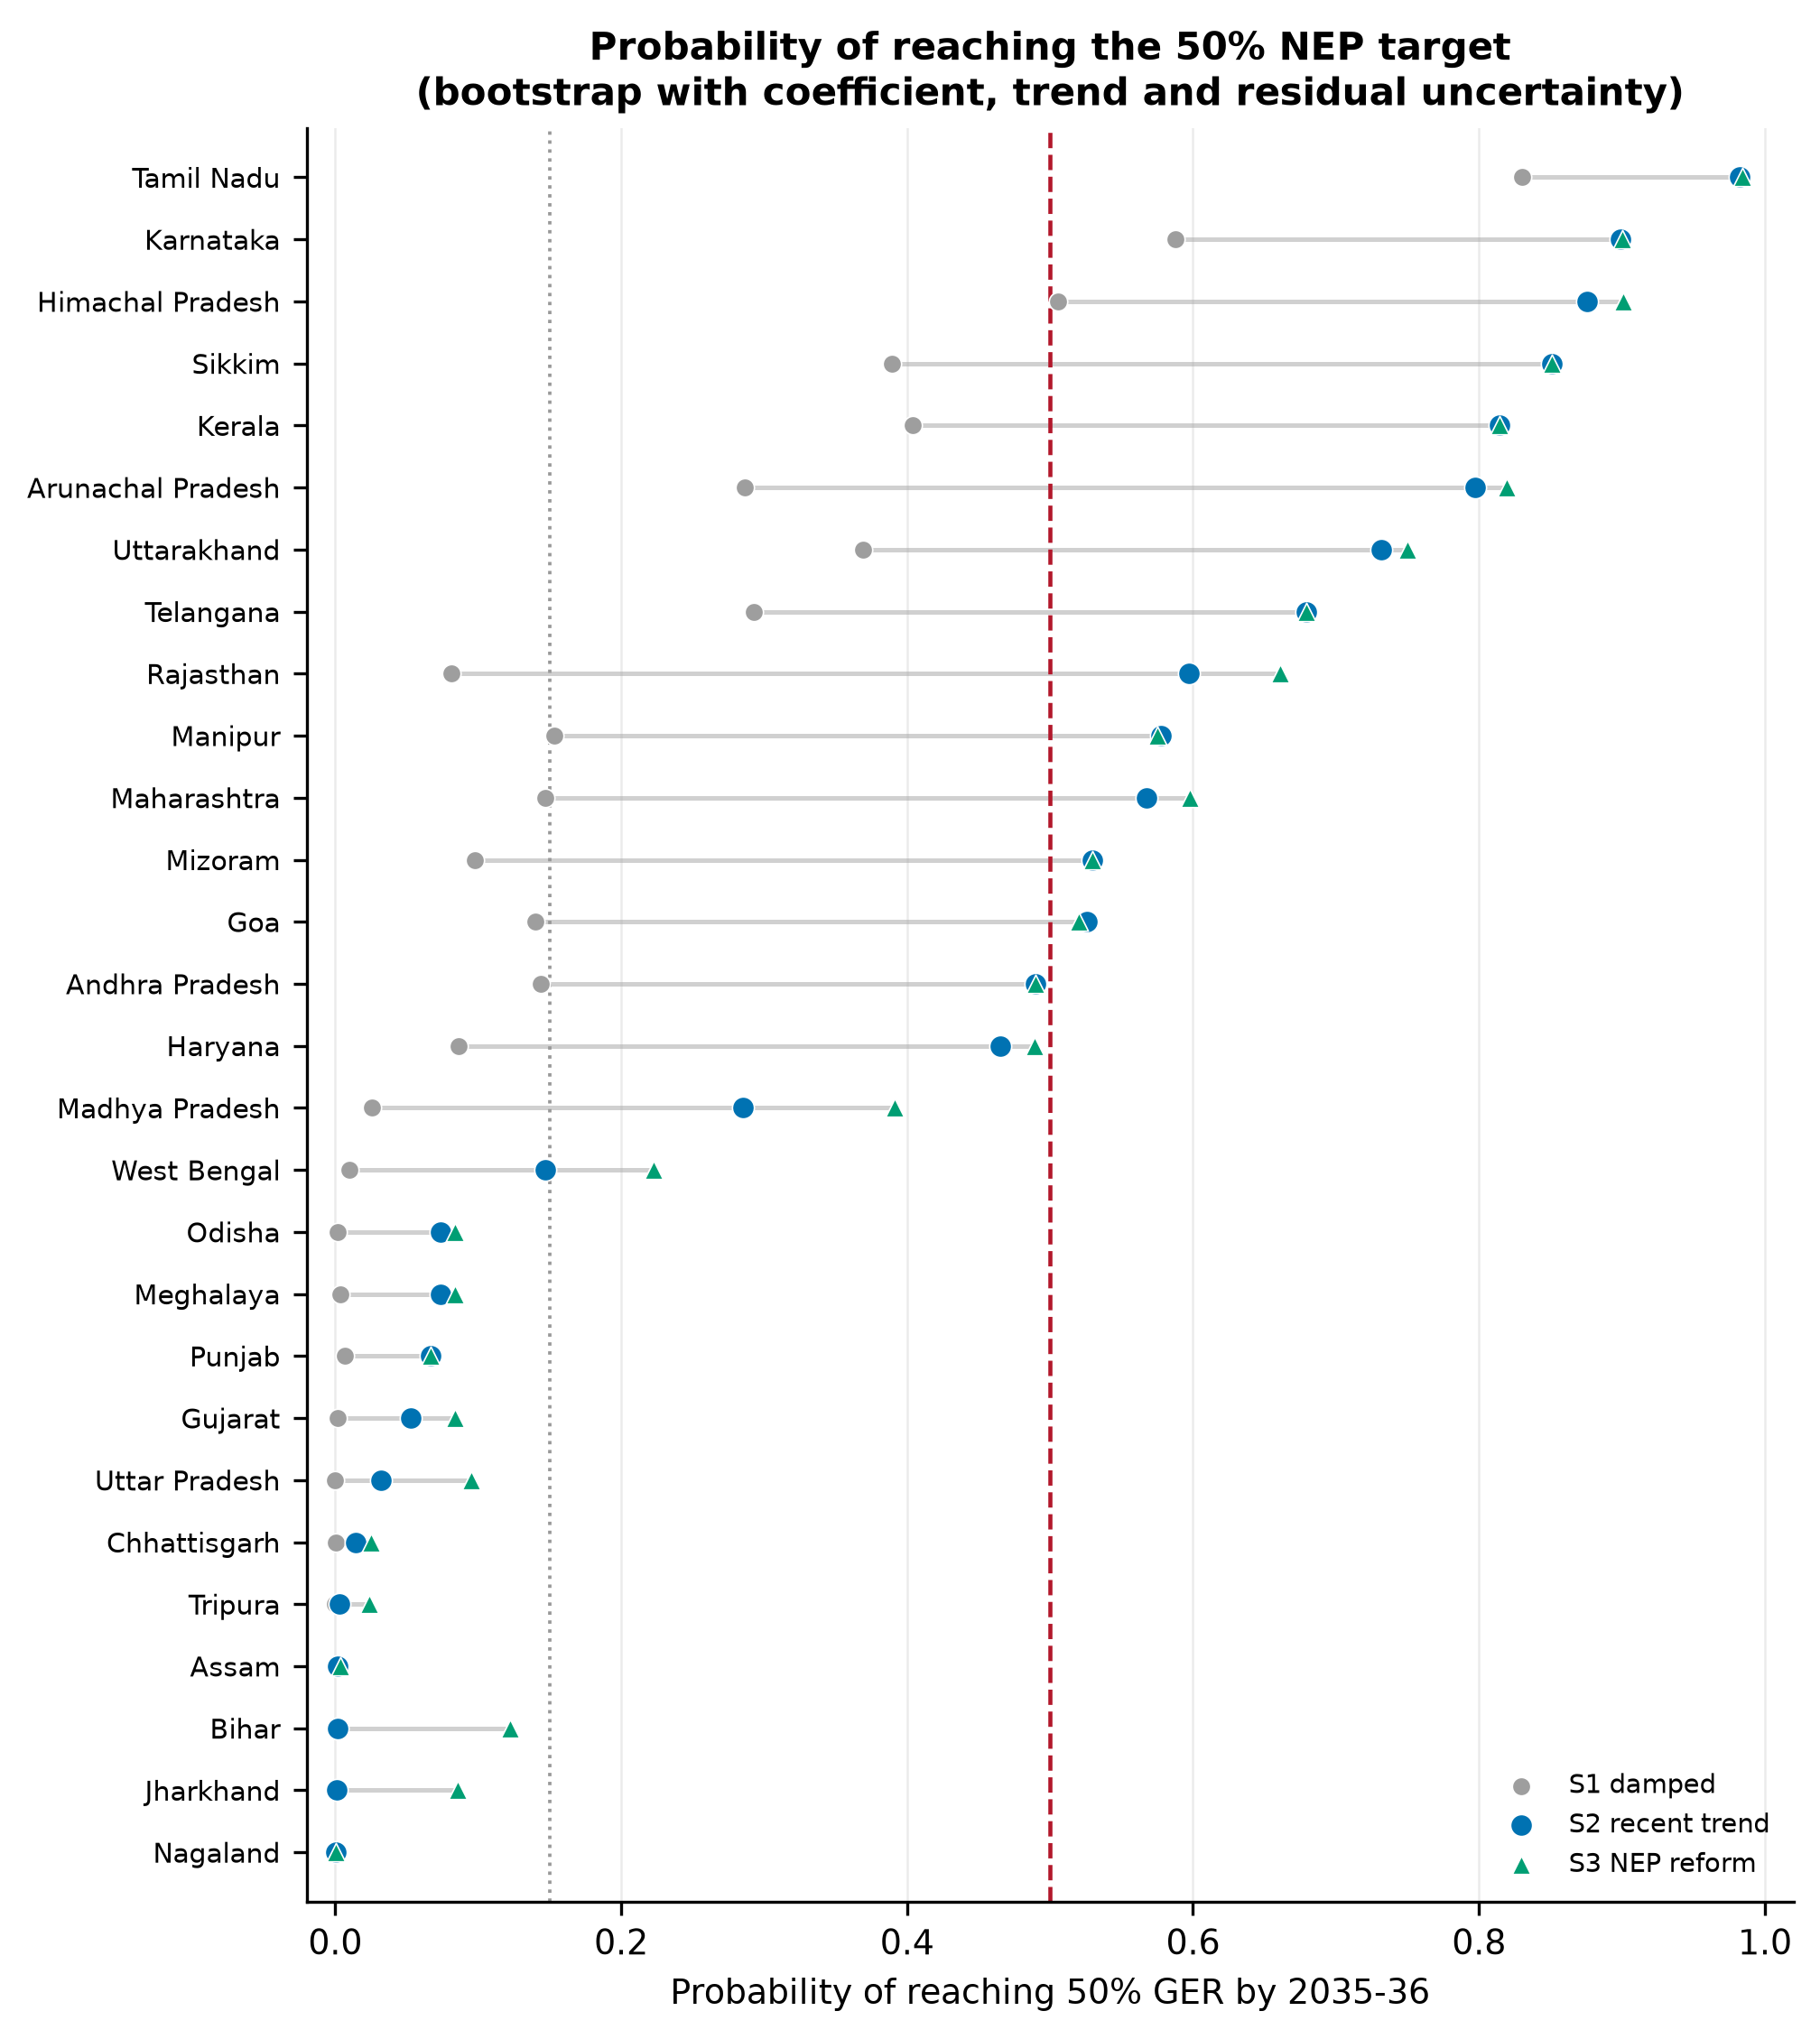
\includegraphics[width=\linewidth]{fig13_probability_reaching_50.png}
\caption{Probability of reaching 50\% by 2035-36 under the three scenarios, 28 States. The 0.5 and 0.15 lines mark the on-track and at-risk thresholds. Source: \texttt{fig13\_probability\_reaching\_50.png}.}
\label{fig:prob50}
\end{figure}

\begin{figure}[htbp]
\centering
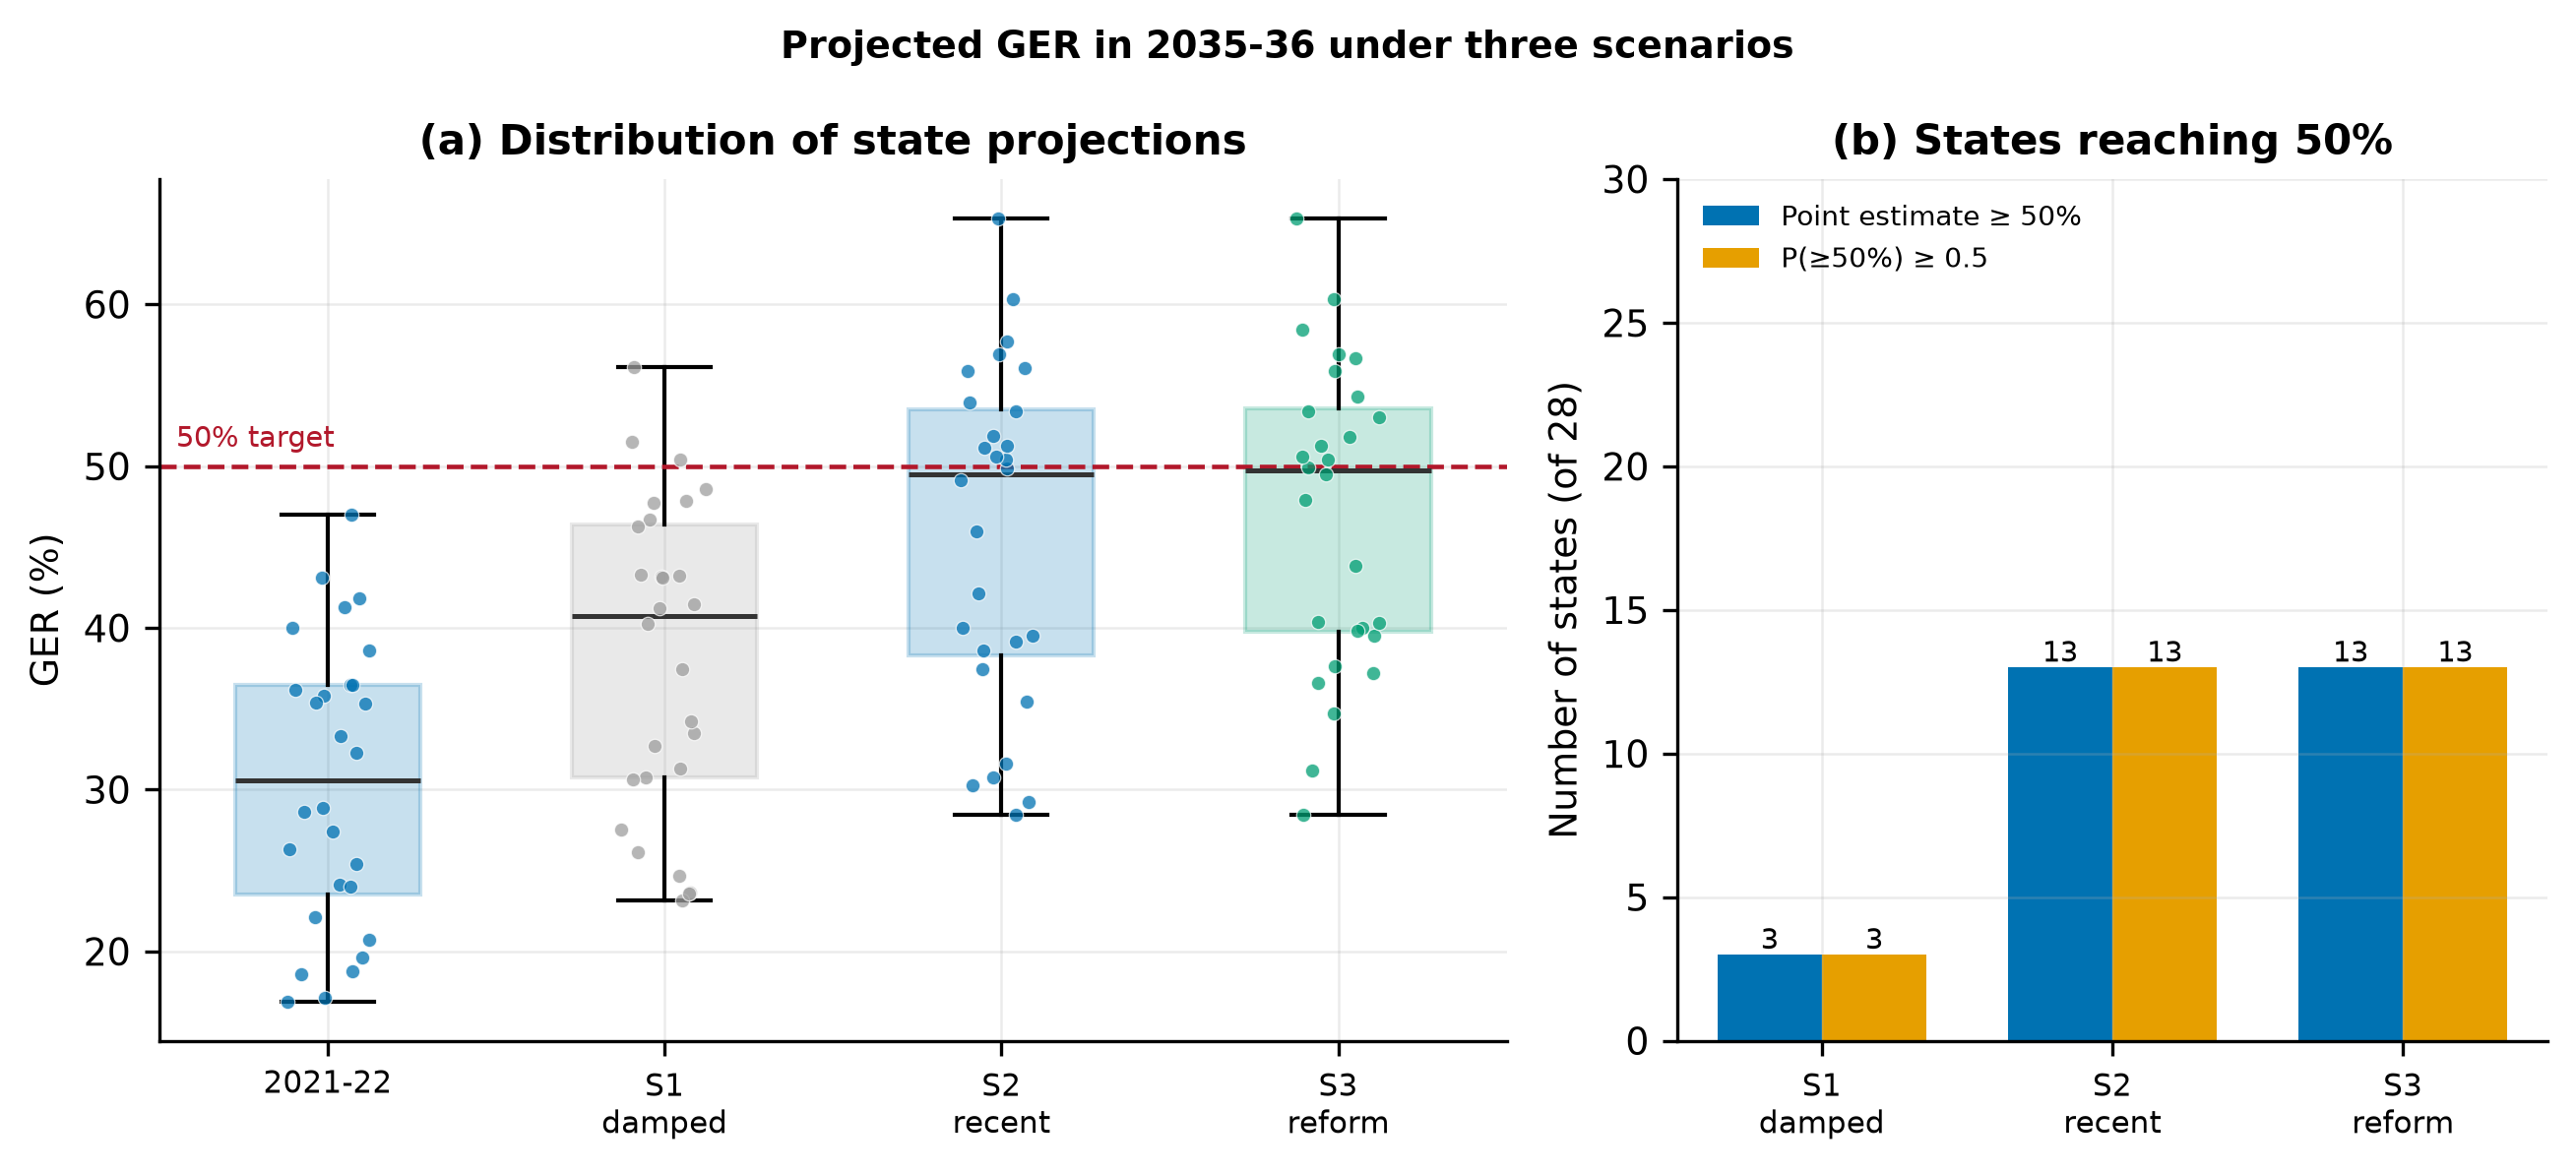
\includegraphics[width=\linewidth]{fig14_scenario_distributions.png}
\caption{Distribution of State projections and the number of States reaching 50\% under each scenario, 28 States. Source: \texttt{fig14\_scenario\_distributions.png}.}
\label{fig:scenariodist}
\end{figure}

Figure~\ref{fig:dumbbell} shows the State-level change and its uncertainty, Figure~\ref{fig:prob50} ranks States by the probability of crossing 50\%, and Figure~\ref{fig:scenariodist} compares the three scenario distributions. The uncertainty is large. For Tamil Nadu, the 5th--95th percentile interval is 53.7 to 77.4; for Bihar it is 17.9 to 40.9. The width reflects three sources: coefficient uncertainty (especially the density coefficient), trend uncertainty (0.866 $\pm$ 0.174 per year) and State-level residual variation (SD \(= 6.31\)). The probability ranking is therefore more informative than a single point forecast.

The population-weighted check is the central result. Using the implied 18--23 population as weights, the 28-State GER rises from 28.0\% in 2021-22 to 35.9\% under S1, 43.5\% under S2 and 45.7\% under S3 in 2035-36. Even the reference scenario leaves the population-weighted GER 6.5 points below the NEP target, and 68.6\% of the 18--23 population lives in States projected below 50\%. The unweighted count of 13 States overstates national progress because the States that are off track are the populous ones.

\subsection{What would it take? Required density}

Table~\ref{tab:required} reports the model-implied college density required by 2035-36 under S2, computed from~\eqref{eq:required} for the ten largest gaps. The required annual changes are far above the observed 2017-22 changes in the low-density States. Bihar would need \(+4.2\) colleges per lakh per year, against an observed change of zero; Uttar Pradesh \(+2.8\) against \(+0.25\); Assam \(+4.2\) against \(+0.25\); Jharkhand \(+3.9\) against zero. Nagaland has the largest gap in college density terms (61.1), but the smallest implied population, so the indicative college requirement is only about 170.

\begin{table}[htbp]
\centering
\caption{Model-implied college density required by 2035-36 under S2, ten largest gaps. \(D_{s,2021}\) is observed college density, \(D_{s,2035}\) is the S2 college density, and \(D_s^{\text{req}}\) is the college density from~\eqref{eq:required} that would deliver 50\% under the model. ``Extra colleges'' multiplies the density gap by the implied 18--23 population; it is an illustration, not a costing. Source: \texttt{table08\_required\_density.csv}.}
\label{tab:required}
\resizebox{\textwidth}{!}{%
\begin{tabular}{@{}lrrrrrrr@{}}
\toprule
State & \(D_{s,2021}\) & \(D_{s,2035}\) & \(D_s^{\text{req}}\) & Gap & Req.\ annual & Obs.\ annual & Extra colleges \\
\midrule
Nagaland & 25 & 18.0 & 79.1 & 61.1 & +3.86 & $-0.50$ & 169 \\
Bihar & 7 & 7.0 & 65.9 & 58.9 & +4.20 & 0.00 & 9,184 \\
Assam & 15 & 18.5 & 74.4 & 55.9 & +4.25 & +0.25 & 2,264 \\
Jharkhand & 8 & 8.0 & 62.6 & 54.6 & +3.90 & 0.00 & 2,499 \\
Tripura & 11 & 7.5 & 59.7 & 52.2 & +3.48 & $-0.25$ & 256 \\
Chhattisgarh & 27 & 37.5 & 78.8 & 41.3 & +3.70 & +0.75 & 1,402 \\
Uttar Pradesh & 29 & 32.5 & 68.0 & 35.5 & +2.79 & +0.25 & 10,262 \\
Gujarat & 32 & 39.0 & 71.3 & 32.3 & +2.81 & +0.50 & 2,419 \\
Odisha & 27 & 41.0 & 71.7 & 30.7 & +3.19 & +1.00 & 1,478 \\
Punjab & 33 & 33.0 & 62.7 & 29.7 & +2.12 & 0.00 & 939 \\
\bottomrule
\end{tabular}}
\end{table}

\begin{figure}[htbp]
\centering
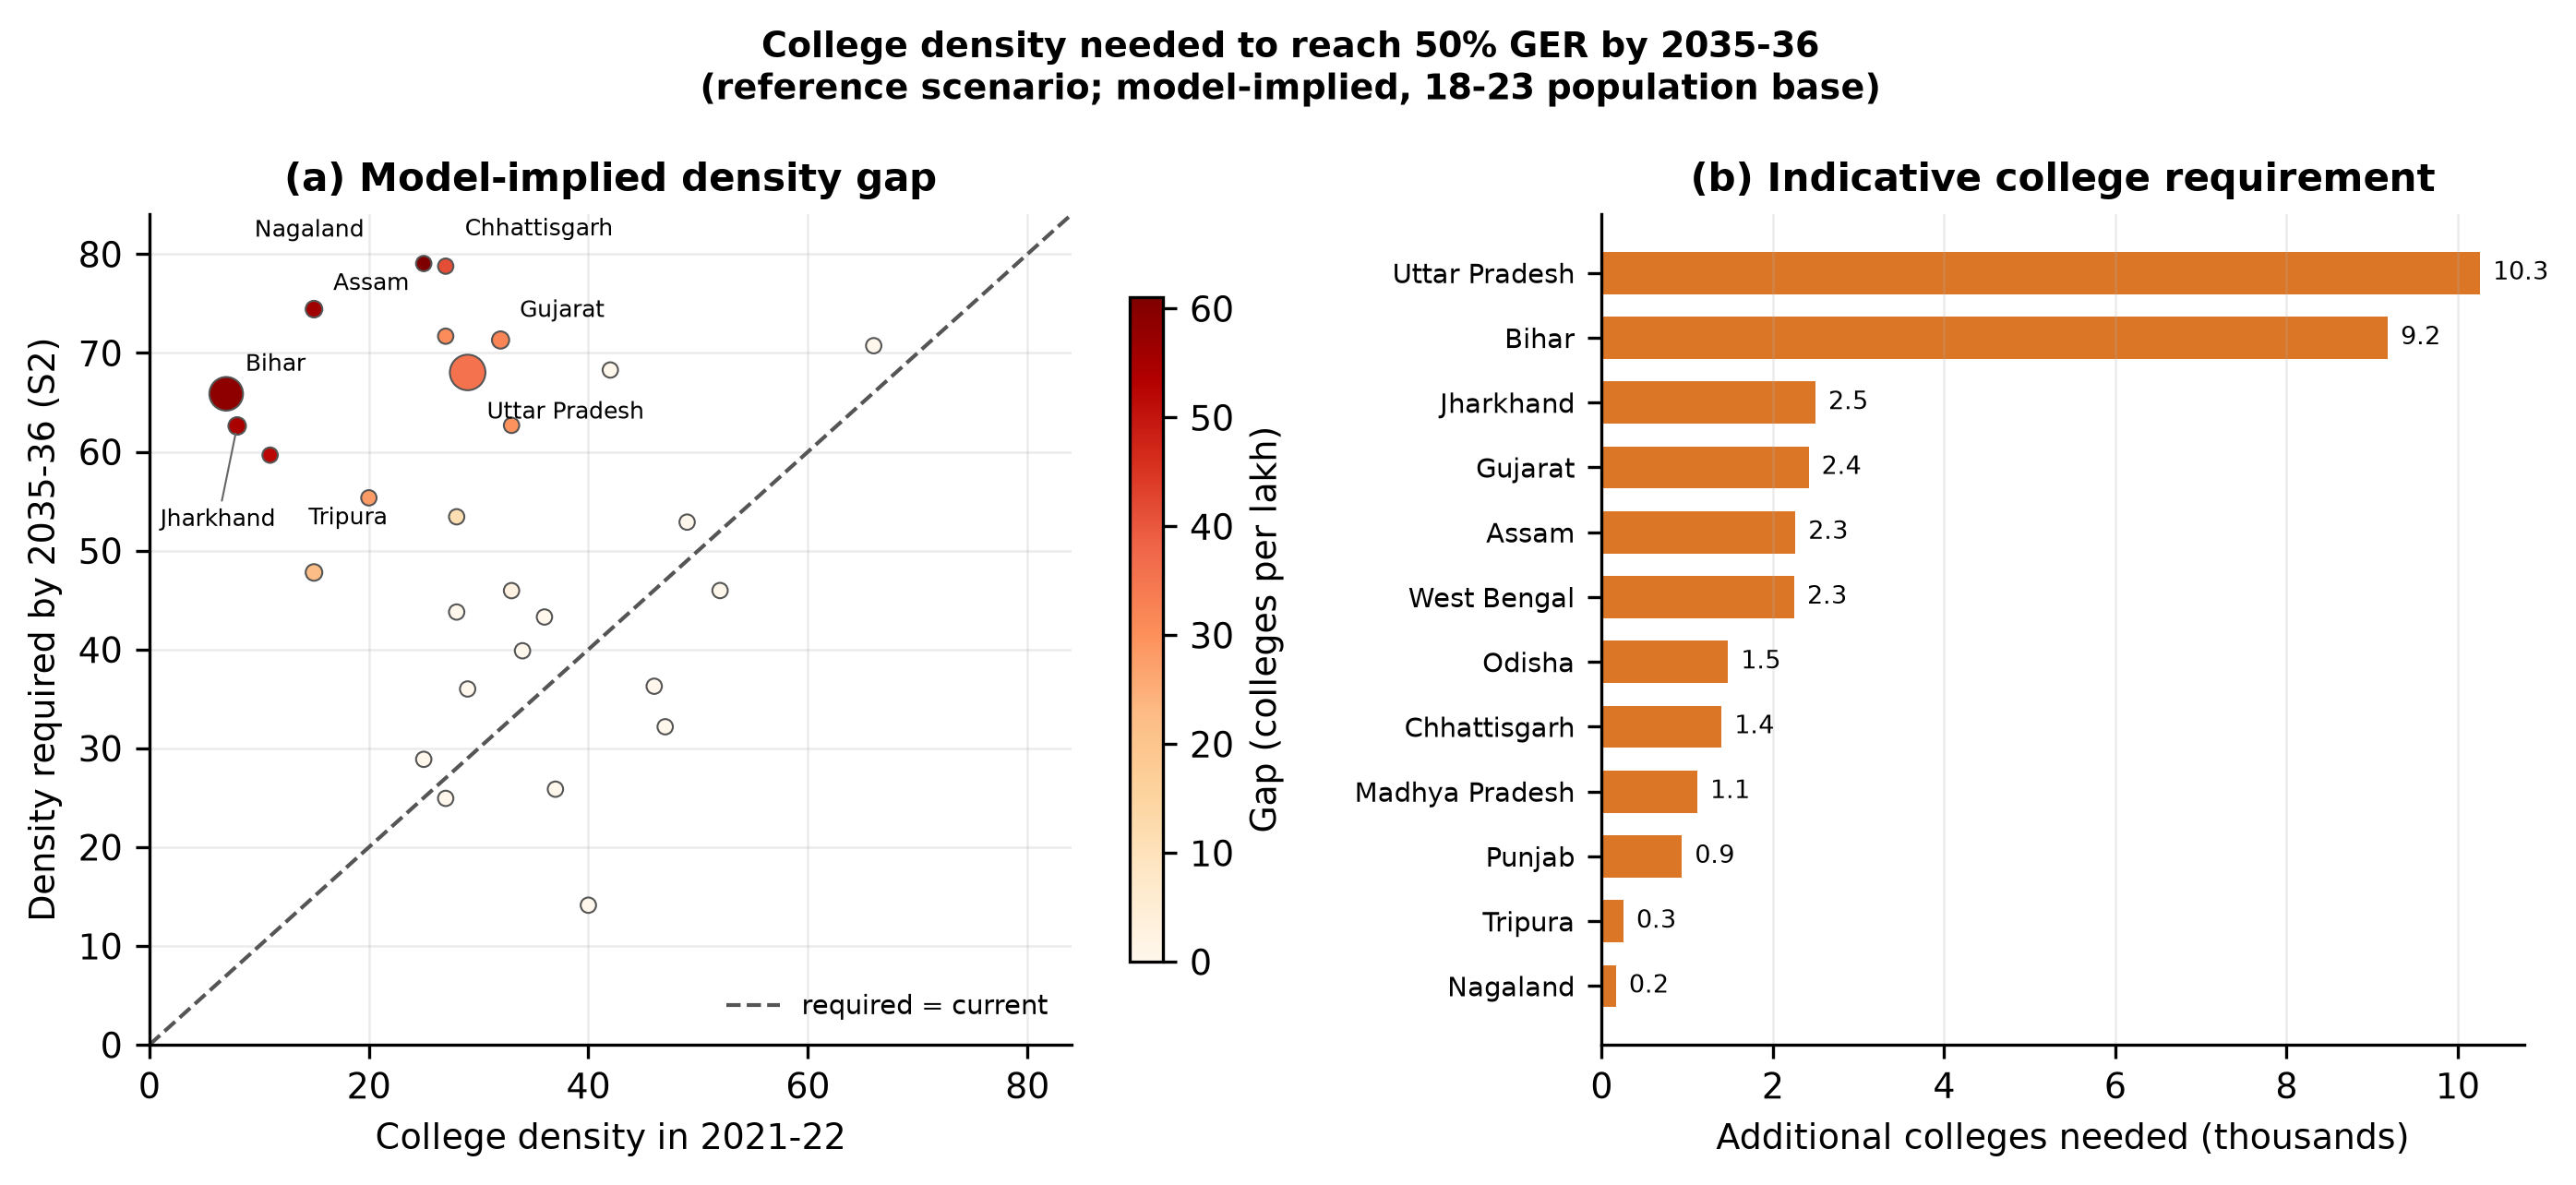
\includegraphics[width=\linewidth]{fig15_required_density.png}
\caption{Model-implied college density required to reach 50\% by 2035-36, and the indicative additional-college requirement, 28 States. Panel (a) plots current density against required density; panel (b) ranks States by the implied number of additional colleges. Source: \texttt{fig15\_required\_density.png}.}
\label{fig:required}
\end{figure}

The indicative additional-college calculation gives the largest figures for Uttar Pradesh (about 10,300), Bihar (about 9,200), Jharkhand (2,500), Gujarat (2,400), Assam (2,300), West Bengal (2,300), Odisha (1,500), Chhattisgarh (1,400) and Madhya Pradesh (1,100). Figure~\ref{fig:required} places the current and required densities side by side. These figures are illustrative. They extrapolate the linear density coefficient far beyond the observed range and ignore teacher supply, funding, land and demand. They should be read as a signal of the scale of the gap, not as a costed plan.

A cautionary comparison is useful. Karnataka already has 66 colleges per lakh, roughly the density the model says Bihar needs, but its GER is 36.2\%, not 50\%. Density is therefore necessary but not sufficient. Demand, quality, programme mix and completion also matter. The required-density figures describe the capacity gap implied by the cross-sectional association; they do not guarantee that reaching that density will deliver 50\%.

\subsection{Union Territories}

The UT appendix is indicative only, because UTs were outside the estimation sample. Applying the 28-State coefficients, Chandigarh (64.8) and Puducherry (61.5) are already above 50\%; Delhi (49.0) is projected at 61.1 with \(P = 0.95\); Jammu and Kashmir (24.8) at 34.5 with \(P = 0.01\); the Andaman and Nicobar Islands (22.6) at 39.7 with \(P = 0.08\); and Dadra and Nagar Haveli and Daman and Diu (11.2) at 17.7 with \(P \approx 0\). Ladakh and Lakshadweep are omitted because of missing predictors or an insufficient panel. The UT results should not be used for policy targeting without a separate city-catchment analysis.
